\PassOptionsToPackage{svgnames}{xcolor}
\documentclass[t, english]{beamer}
\usepackage[utf8]{inputenc}
\usepackage[T1]{fontenc}
\usepackage{tikz}
\usepackage[default]{comfortaa}
\usepackage{pgfpages}
\usepackage{listings}
\usepackage{appendixnumberbeamer}

\usetikzlibrary{trees}

\lstset{
  basicstyle=\ttfamily\scriptsize\color{black},
  showstringspaces=false,
  commentstyle=\color{red},
  keywordstyle=\color{blue},
  language=bash,
  backgroundcolor=\color{white},
}

%\pgfpagesuselayout{8 on 1}[a4paper, border shrink=5mm]
\setbeameroption{show notes on second screen=bottom}
%\setbeameroption{hide notes}
%%\setbeameroption{show notes}

\setbeamertemplate{note page}[plain]
\beamertemplatenavigationsymbolsempty

\synctex=1
\hypersetup{pdfpagemode=UseNone} % don't show bookmarks on initial view
\usetheme{default}
\usefonttheme{professionalfonts}

\setbeamertemplate{footline}{%
\raisebox{5pt}{%
\makebox[\paperwidth]{%
\hfill\makebox[25pt]{%
\scriptsize\insertframenumber/\inserttotalframenumber%
}%
}%
}\hspace*{5pt}%
}

\begin{document}

\title{Etude et réalisation du serveur de la nouvelle plate-forme CosyVerif}
\author{Idrissa SOKHONA}
\date{29 Septembre 2014}

\begin{frame}
\begin{center}

\par
\Huge Conception et réalisation du serveur de la nouvelle plate-forme CosyVerif

\par
\normalsize
\textsf{Idrissa SOKHONA}

\par
\textsf{idrissa.sokhona@etu.upmc.fr}

\par
\textsf{Université Pierre et Marie Curie,}

\par
\textsf{Master informatique,}

\par
\textsf{Spécialité SAR, Parcours SRETR}

\begin{tikzpicture}
    \node
      [anchor=north]
      at (1,3)
      {
\includegraphics[height=2cm]{img/lipn}};
    \node
      [anchor=north]
      at (6.5,3)
      {
\includegraphics[height=2cm]{img/lsv}};
  \end{tikzpicture}
\end{center}
\end{frame}

\begin{frame}[c]
  \frametitle{Context}
  
  \begin{minipage}{1\textwidth}
  	\only <1>{%
                \begin{tikzpicture}
                      \node
                          [anchor=north]
                          at (0,0)
                          {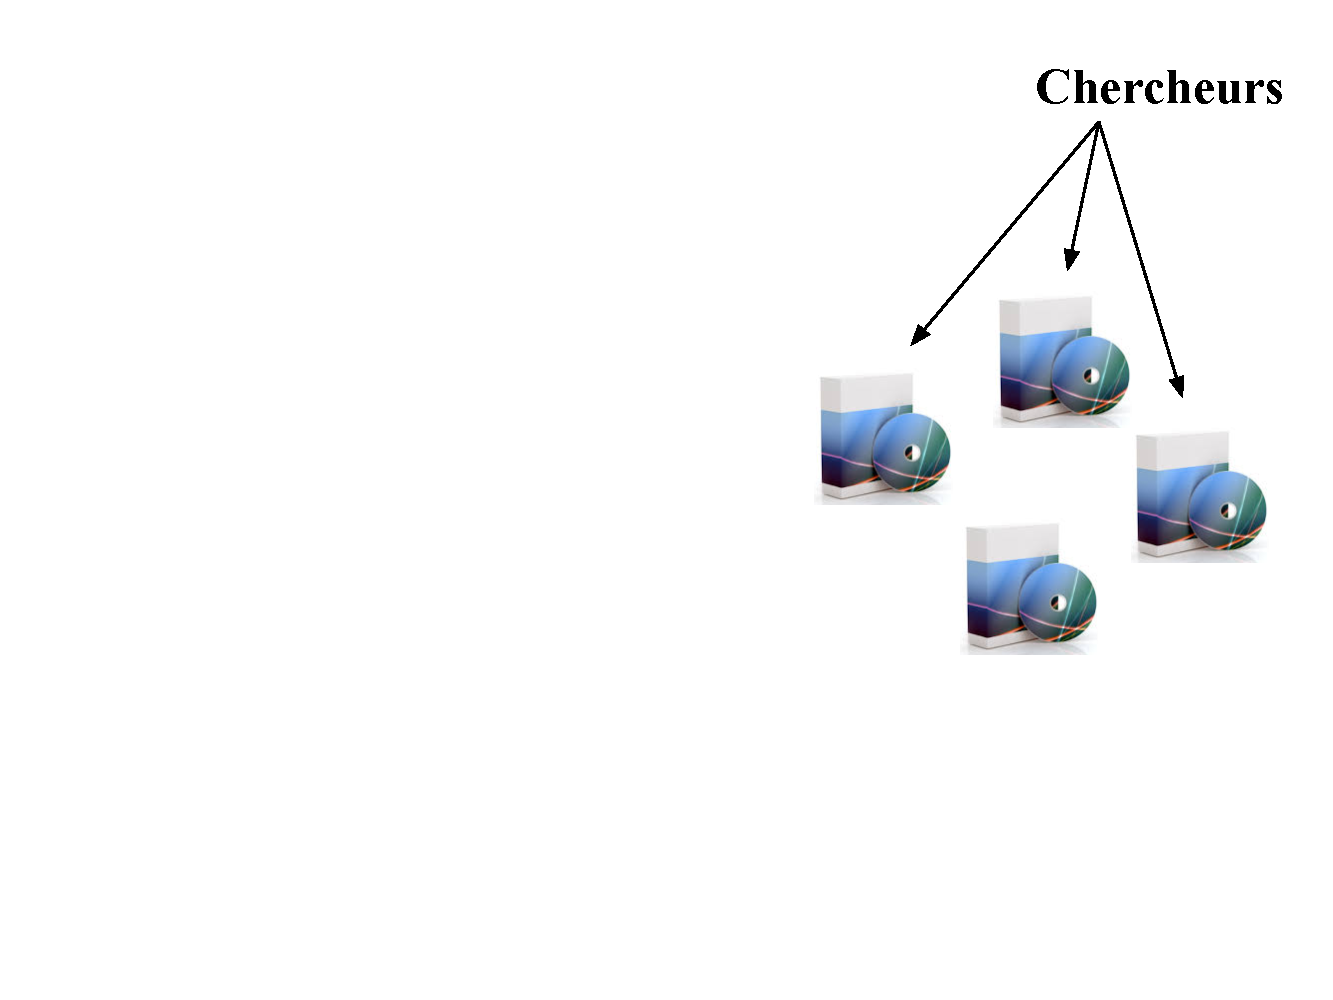
\includegraphics[width=10.5cm, height=4cm]{img/1-chercheur}};
                 \end{tikzpicture}
            }%
            
            \only <2-7>{%
                \begin{tikzpicture}
                      \node
                          [anchor=north]
                          at (0,0)
                          {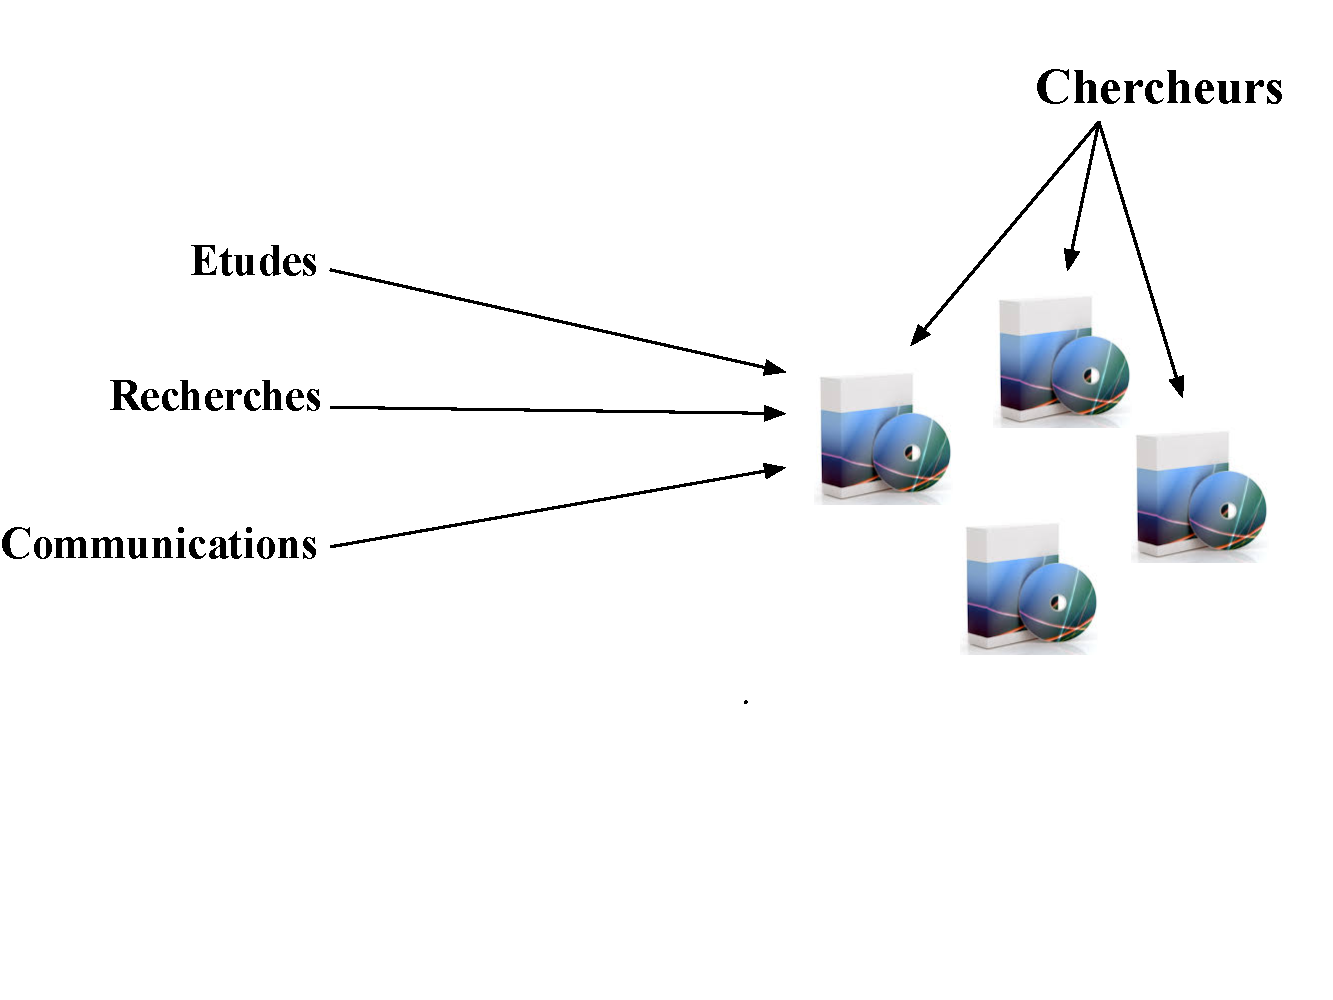
\includegraphics[width=10.5cm, height=4cm]{img/2-chercheur}};
                 \end{tikzpicture}
            }%
            
            \only <8>{%
                \begin{tikzpicture}
                      \node
                          [anchor=north]
                          at (0,0)
                          {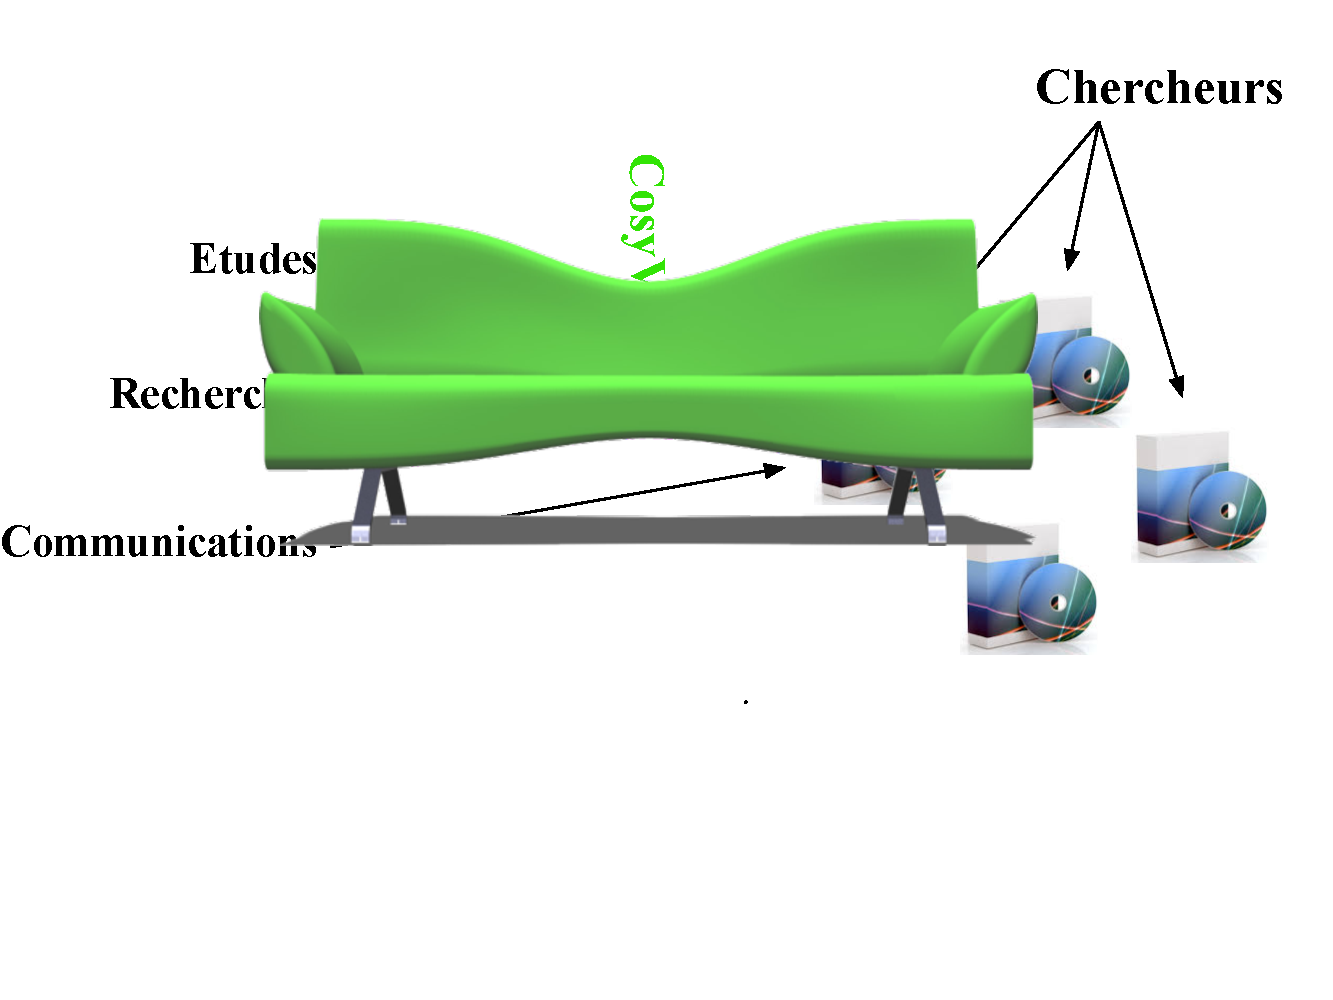
\includegraphics[width=10.5cm, height=4cm]{img/3-chercheur}};
                 \end{tikzpicture}
            }%
            
            \only <9>{%
                \begin{tikzpicture}
                      \node
                          [anchor=north]
                          at (0,0)
                          {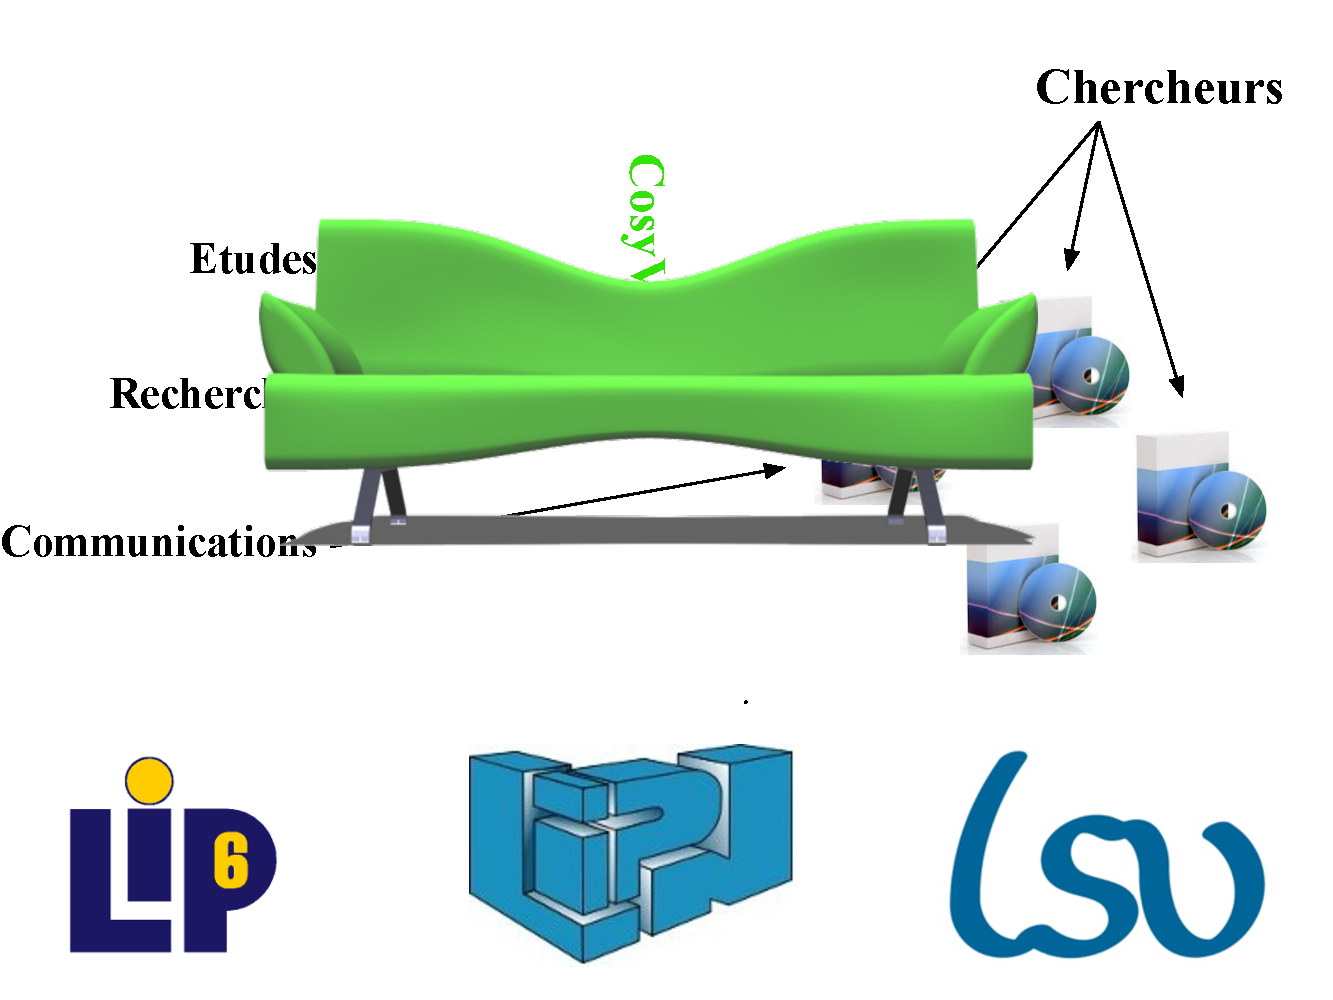
\includegraphics[width=10.5cm, height=4cm]{img/4-chercheur}};
                 \end{tikzpicture}
            }%
 
    \end{minipage}
   
   \hrule
  
  \begin{minipage}{1\textwidth}
    
         \begin{itemize}
     	    \item <3->Installer
     	    \item <4->Prise en main
	    \item <5->Format d'entrée
     	    \item <6->Format de sortie
     	    \item <7->Analyse de résultats
         \end{itemize}
   \end{minipage}

   \note{
    \begin{itemize}
     \item CosyVerif est une collection d'outils
     \item Ces outils sont utilisés à plusieurs occasions :
       \begin{itemize}
         \item Enseignement, par exemple le cours ??? de Fabrice Kordon
               en M2 SAR
         \item Communication, par exemple lors des démonstrations d'outils
               dans les conférences, ou les portes ouvertes du LSV
         \item Projets, par exemple lors du projet européen MIDAS
       \end{itemize}
     \item Ces outils sont écrits par des chercheurs
     \item Ces outils sont dédiés à des calculs très pointus
     \item Mais les chercheurs n'ont pas de temps à consacrer à leur peaufinage
     \item Les outils sont donc généralement difficiles à utiliser :
       \begin{itemize}
         \item Difficulté d'installation, par exemple GreatSPN a nécessité
           deux demies-journées pour arriver à l'installer
         \item Difficulté de prise en main, souvent en ligne de commande,
           aide plus ou moins existante
         \item Formats d'entrée très variables, souvent propre à l'outil,
           par exemple Prod, GreatSPN... un format standardisé PNML pas
           toujours supporté
         \item Format de sortie propre à chaque outil, souvent texte
         \item Analyse des résultats pas évidente, par exemple vérifier la
           présence de deadlock avec Prod ne répond pas juste oui/non
       \end{itemize}
     \item CosyVerif aide à utiliser les outils :
       \begin{itemize}
         \item En empaquetant les outils
         \item En fournissant un format unique d'entrée / sortie
         \item En fournissant une méthode unique d'interaction avec les
           outils
         \item En fournissant différents clients permettant d'interagir avec
           le serveur
       \end{itemize}
   \end{itemize}
   Transition: comment?
   }
 \end{frame}

\begin{frame}
\only<1-3>{
  \frametitle{État actuel}
}\only<4-7>{
  \frametitle{Problèmes}
}\only<8->{
  \frametitle{Évolutions}
}
\begin{tikzpicture}
\node (c1) at (2,3)
  {
\includegraphics[width=3cm,height=3cm]{img/screen}};
\node (c2) at (2,7)
  {
\includegraphics[width=3cm,height=3cm]{img/screen}};
\node at (2,5)
  {Clients};
\node (s) at (7,5)
  {
\includegraphics[width=3cm,height=3cm]{img/screen}};
\only<5-7>{
\node [anchor=center]
  at (s.south)
  {
\includegraphics[width=1cm]{img/java2}};
}
\only<8->{
\node [anchor=center]
  at (s.south)
  {
\includegraphics[width=1cm]{img/php.png}};
}
\only<7->{
  \node [anchor=north west] at (s.east)
  {
\includegraphics[width=1cm]{img/depot2}?};
}
\only<6->{
  \node [anchor=north west] at (s.north east)
  {
\includegraphics[width=1cm]{img/users}?};
}
\node at (7,3)
  {Server};
\only<1-4>{
\node
  at (2, 3.3)
  {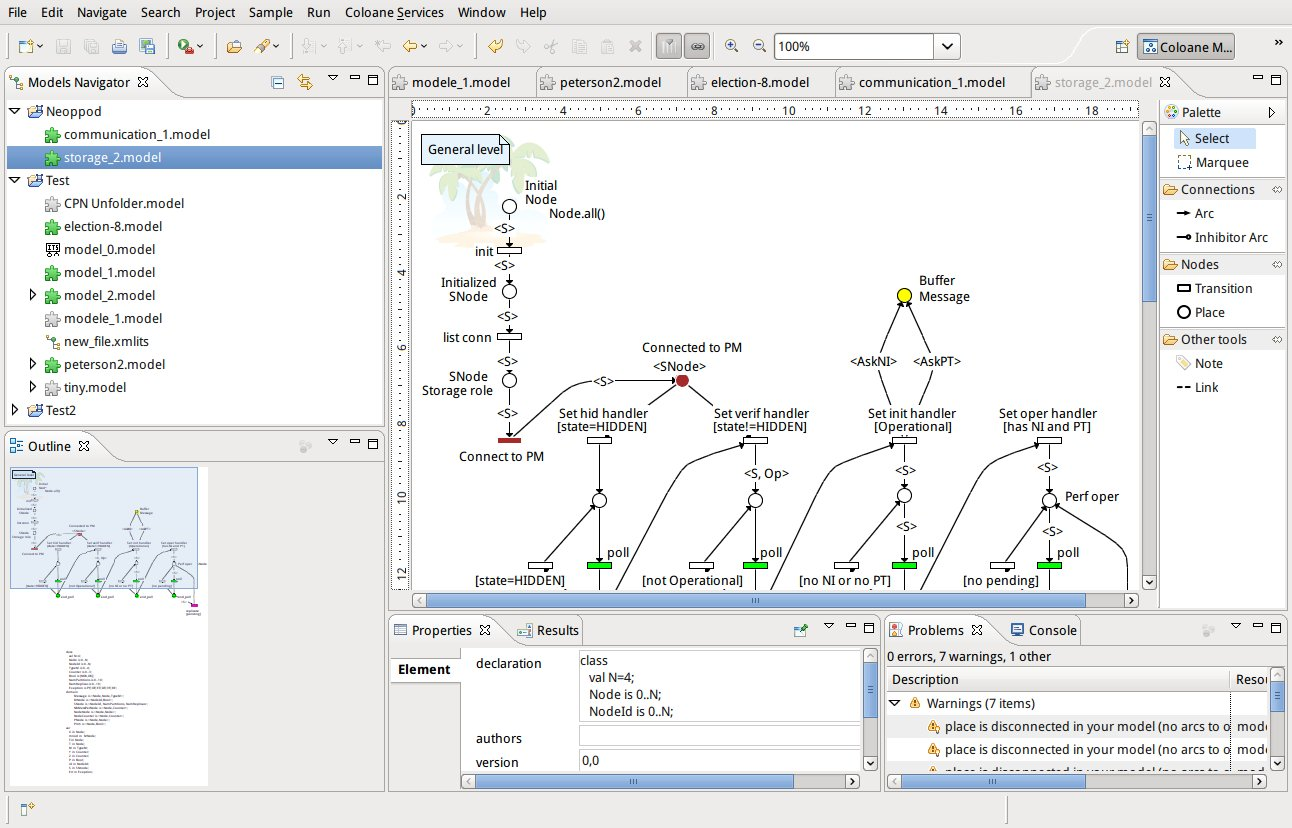
\includegraphics[width=2.8cm,height=2.2cm]{img/coloane-screenshot}};
}
\only<4-7>{
\node (coloane)
  at (2, 3.3)
  {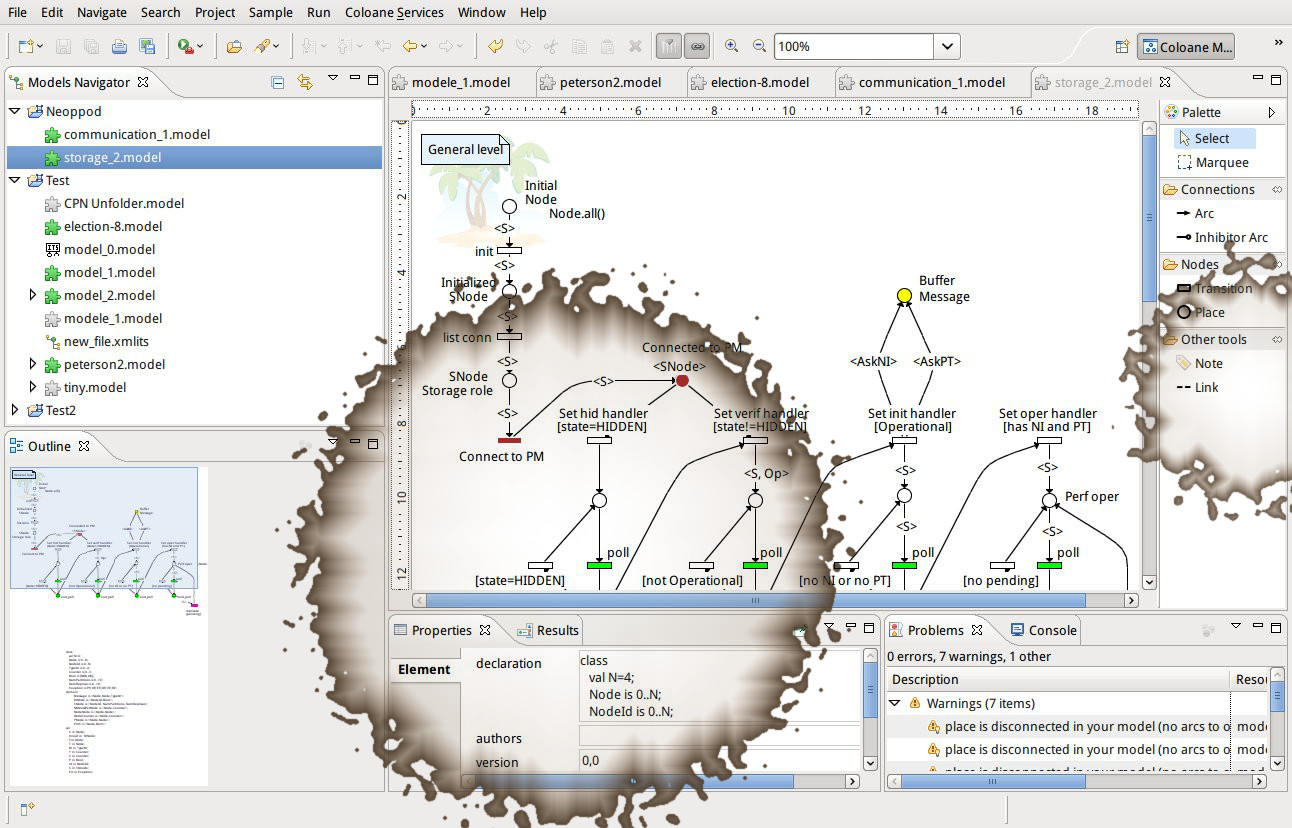
\includegraphics[width=2.8cm,height=2.2cm]{img/coloane-deprecated}};
\node [anchor=north]
  at (coloane.south)
  {
\includegraphics[width=1cm]{img/eclipse}};
}
\only<7->{
\node (coloane)
  at (2, 3.3)
  {\color{white}?};
}
\node
  at (2, 7.3)
  {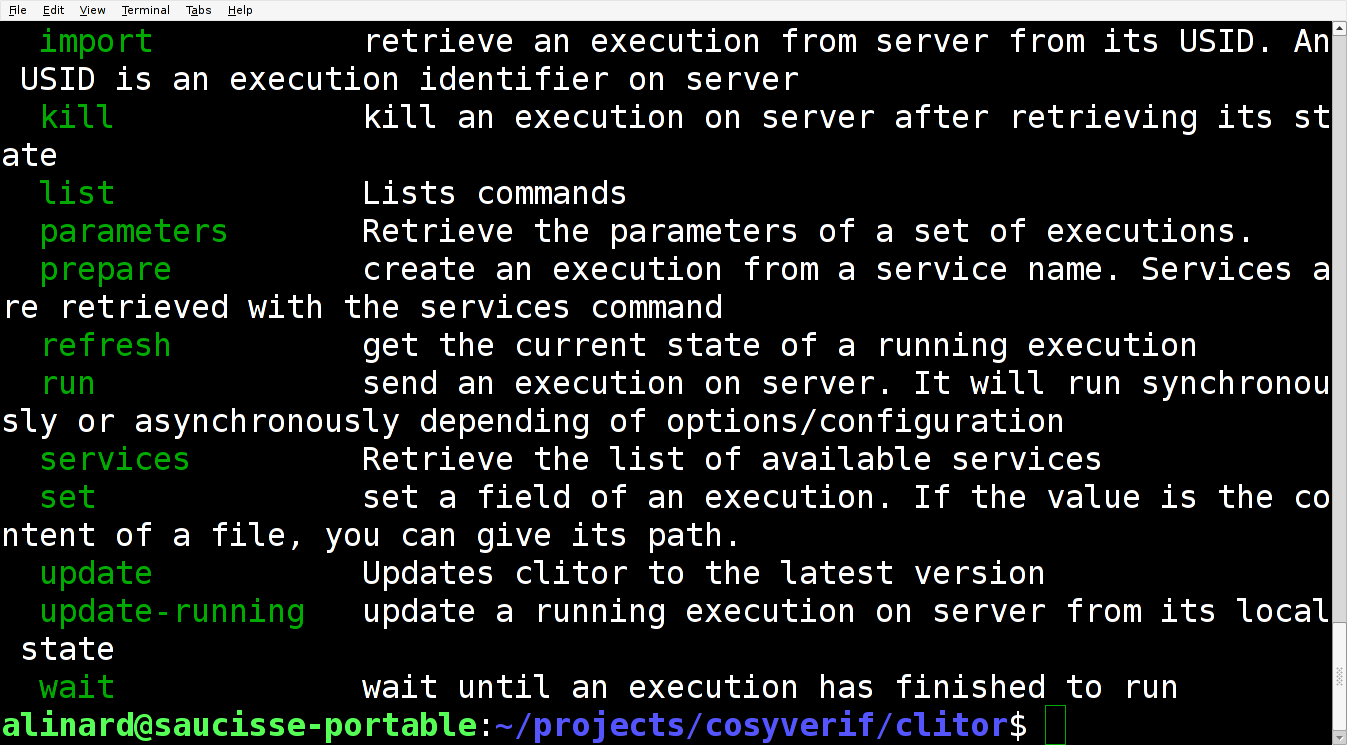
\includegraphics[width=2.8cm,height=2.2cm]{img/clitor}};
\node (t1)
  at (6.5, 5)
  {
\includegraphics[height=1cm]{img/tools-1}};
\node (t2)
  at (7.5, 5.5)
  {
\includegraphics[height=1cm]{img/tools-2}};
\only<1>{
\draw [<->, line width=2pt]
  (c1) -- (s);
\draw [<->, line width=2pt]
  (c2) -- (s);
}
\only<3-7>{
\draw [<->, line width=2pt]
  (c1) -- (s)
  node [midway, below, sloped] {SOAP};
\draw [<->, line width=2pt]
  (c2) -- (s)
  node [midway, above, sloped] {SOAP};
}
\only<8->{
\draw [<->, line width=2pt]
  (c1) -- (s)
  node [midway, below, sloped] {REST};
\draw [<->, line width=2pt]
  (c2) -- (s)
  node [midway, above, sloped] {REST};
}
\only<2>{
\draw [<->, line width=2pt]
  (c1) -- (s.west)
  node [midway, below, sloped] {GrML};
\draw [<->, line width=2pt]
  (c2) -- (s.west)
  node [midway, above, sloped] {GrML};
\draw [<->, color=DarkGreen, line width=2pt]
  (s.west) -- (t2.center)
  node [midway, above, sloped] {
    \tiny\color{white} GrML $\leftrightarrow$ ?
  };
}
\end{tikzpicture}

\note{
  \begin{itemize}
    \item Architecture client/serveur
    \item Deux types de clients : ligne de commande et client/éditeur
      graphique
    \item Un serveur qui embarque les outils
    \item Format d'échange GrML
    \item Problème \#1: protocole de communication SOAP
      \begin{itemize}
        \item Adapté aux projets industriels
        \item Lourd, nécessite une bibliothèque complexe
        \item Clients difficiles à écrire, par exemple le client en ligne de
          commande écrit en PHP a rencontré des difficultés
      \end{itemize}
    \item Problème \#2: maintenance du client Coloane
      \begin{itemize}
        \item Plug-in Eclipse
        \item Pas de permanent disposant de ces compétences dans CosyVerif
        \item Coût d'entrée trop élevé pour les stagiaires
      \end{itemize}
    \item Problème \#3: évolution du serveur
      \begin{itemize}
        \item Écrit en Java
        \item Repose sur des bibliothèques complexes (WebServices)
        \item Pas de permanent disposant de ces compétences dans CosyVerif
        \item Des fonctionnalités simples et nécessaires (utilisateurs,
          dépôt) prennent trop de temps à déveloper
      \end{itemize}
  \end{itemize}
}
\end{frame}
 
 \begin{frame}[c]
  \frametitle{Problématique}
  
  \begin{minipage}{1\textwidth}
  	\only <1>{%
                \begin{tikzpicture}
                      \node
                          [anchor=north]
                          at (0,0)
                          {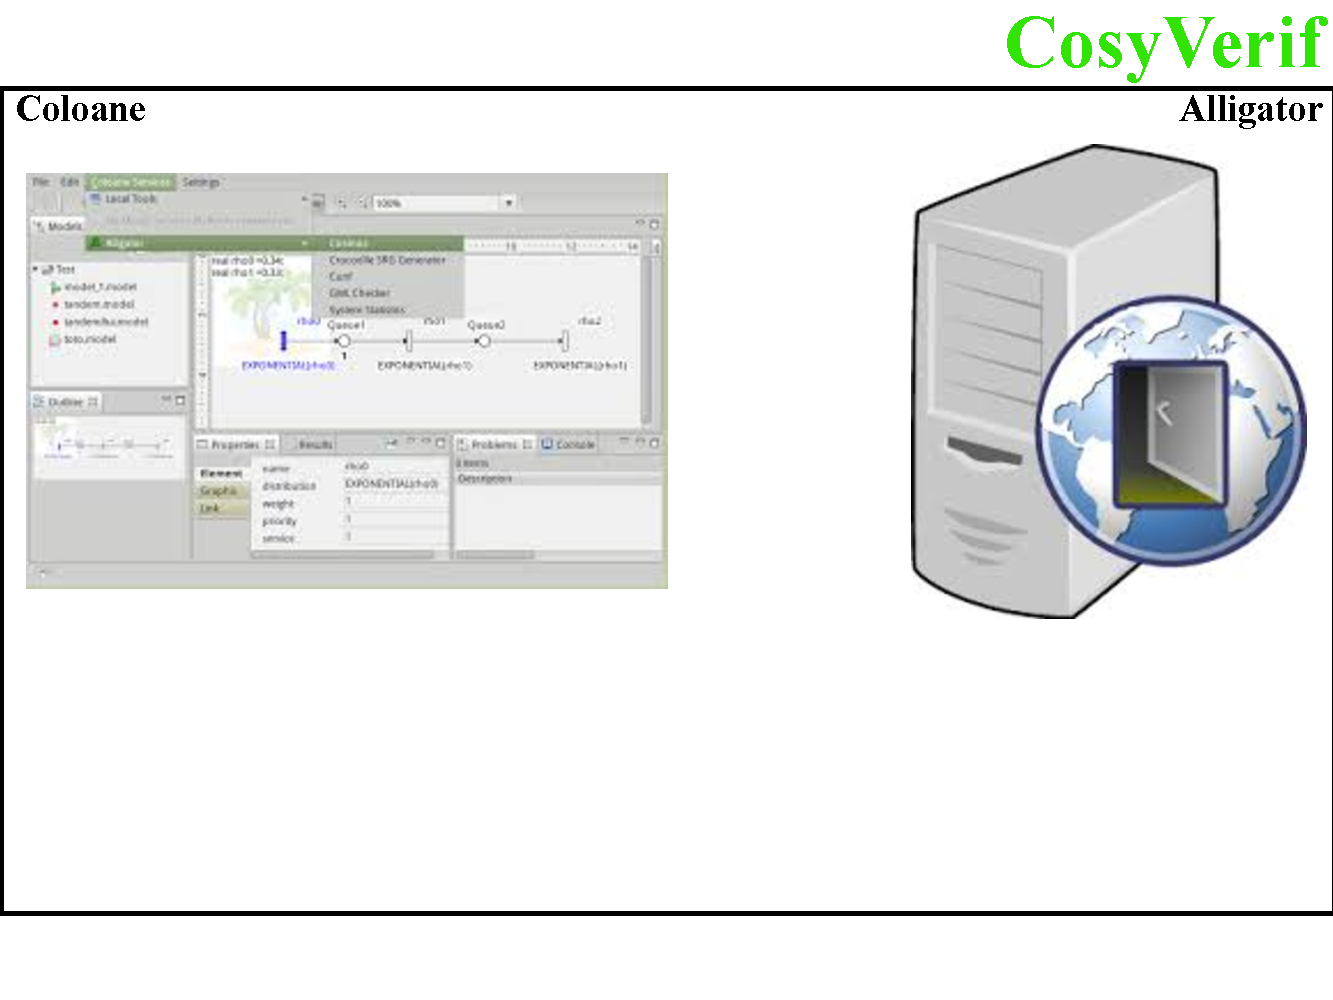
\includegraphics[width=10.5cm, height=4cm]{img/1-probleme}};
                 \end{tikzpicture}
            }%
            
            \only <2>{%
                \begin{tikzpicture}
                      \node
                          [anchor=north]
                          at (0,0)
                          {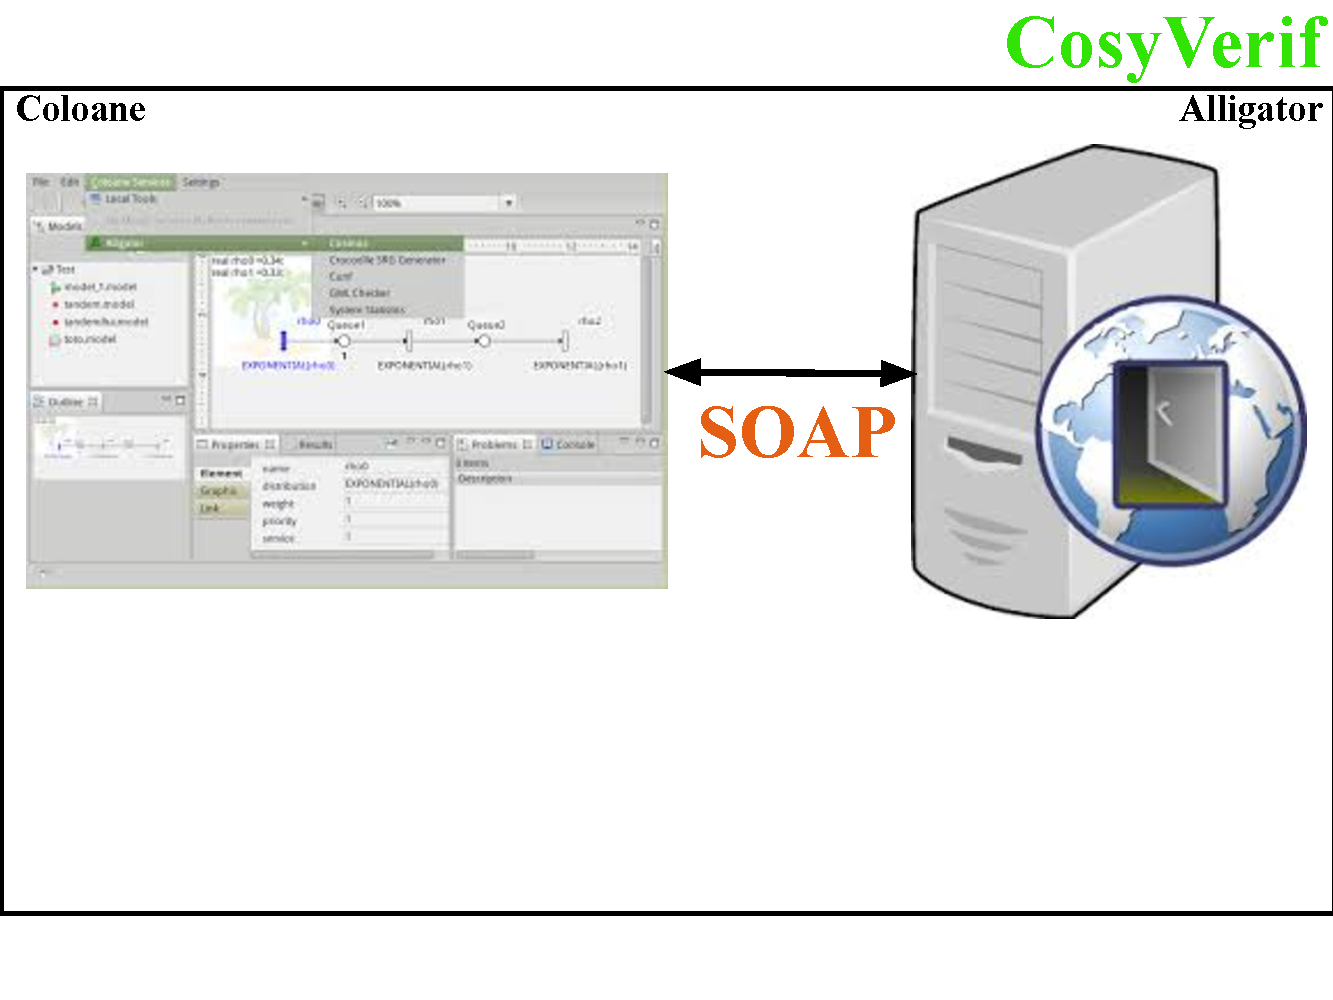
\includegraphics[width=10.5cm, height=4cm]{img/2-probleme}};
                 \end{tikzpicture}
            }%
            
            \only <3>{%
                \begin{tikzpicture}
                      \node
                          [anchor=north]
                          at (0,0)
                          {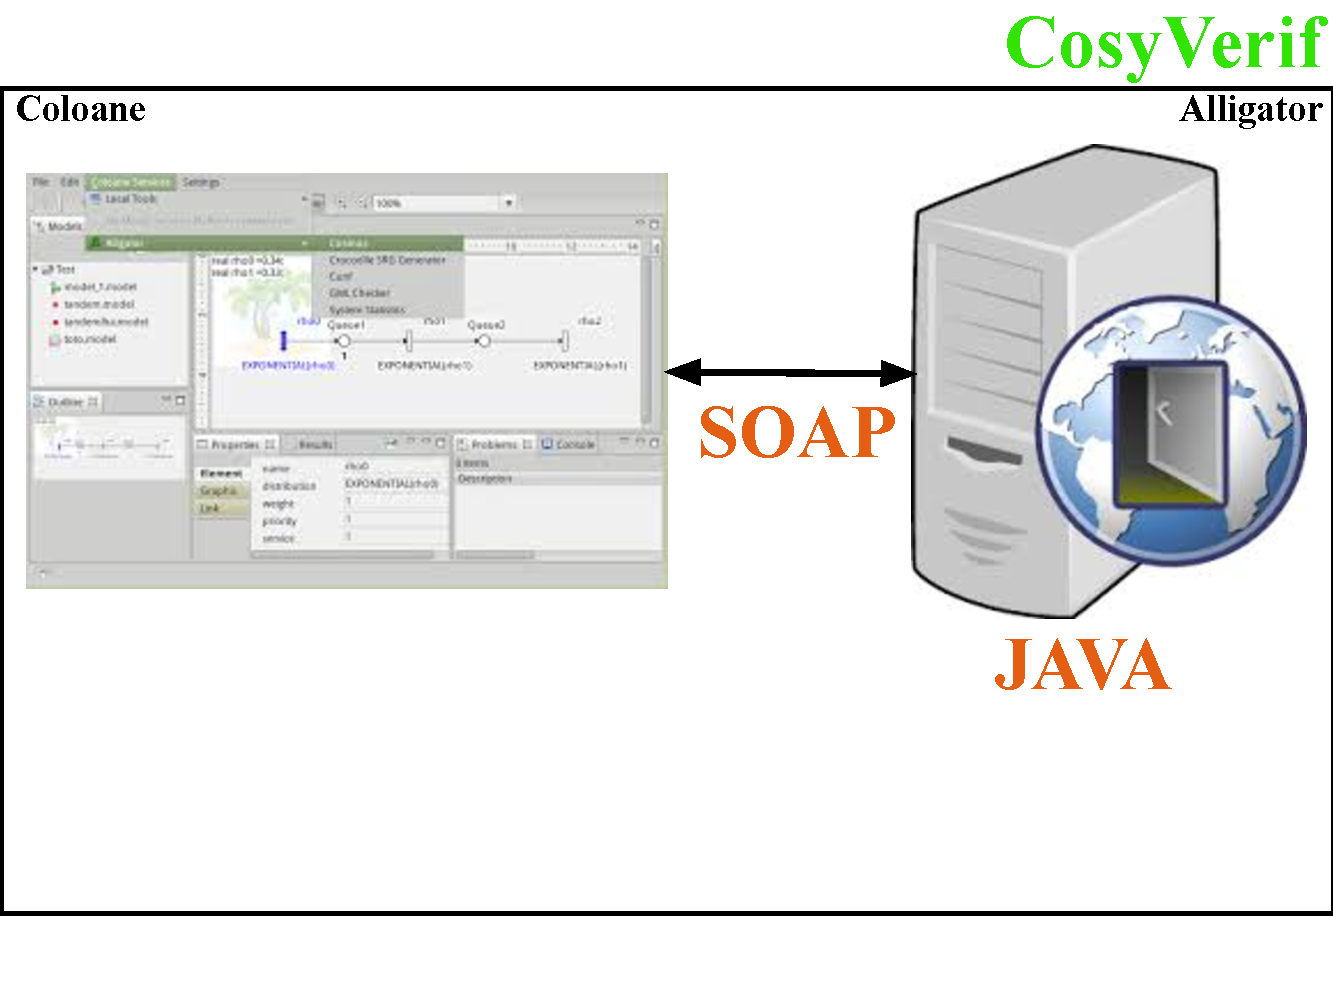
\includegraphics[width=10.5cm, height=4cm]{img/3-probleme}};
                 \end{tikzpicture}
            }%
            
            \only <4>{%
                \begin{tikzpicture}
                      \node
                          [anchor=north]
                          at (0,0)
                          {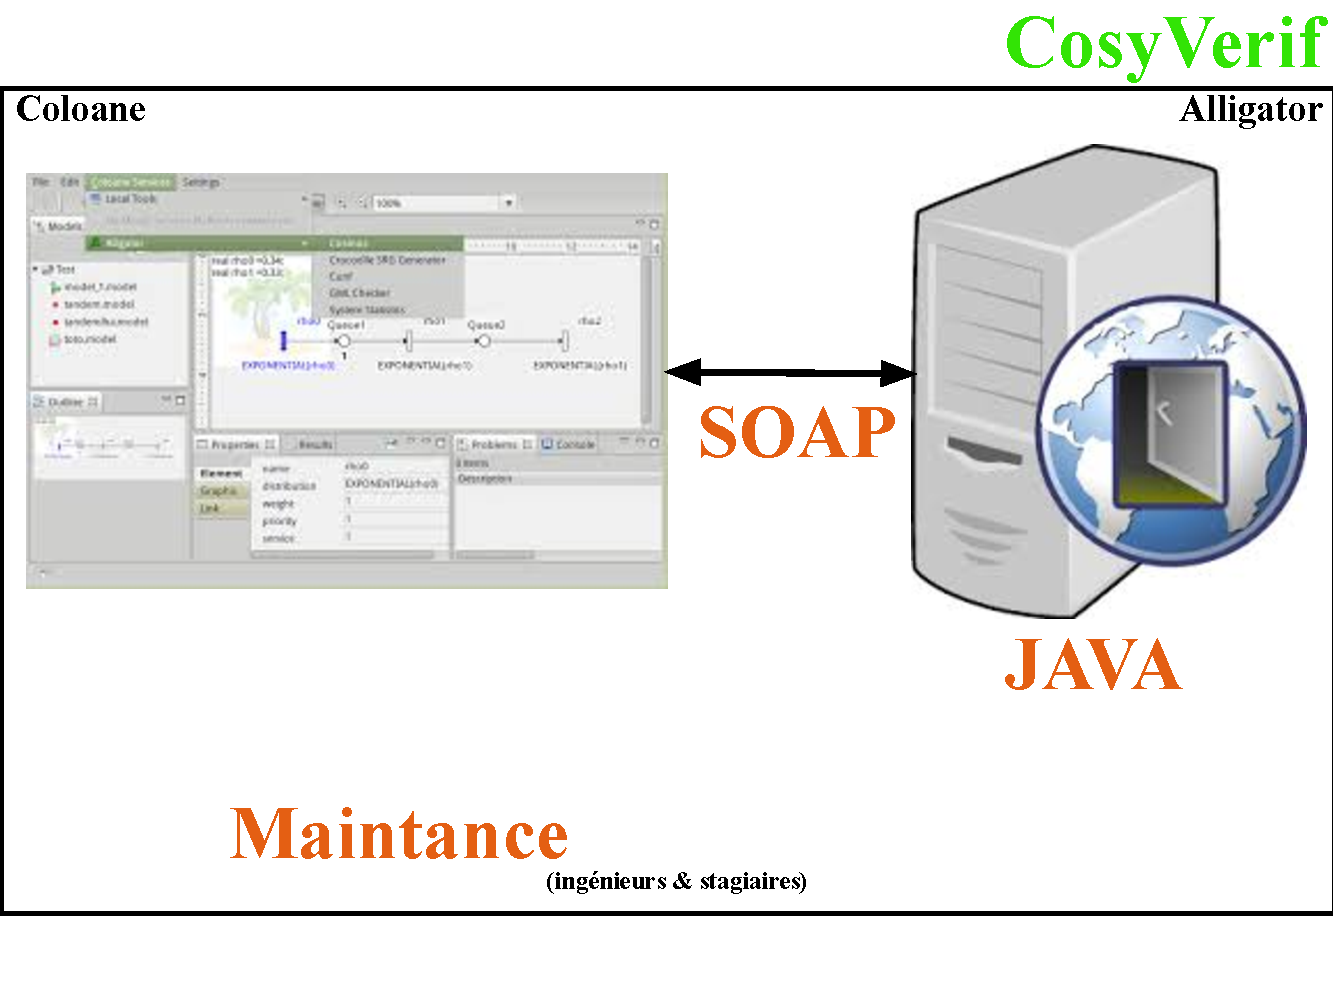
\includegraphics[width=10.5cm, height=4cm]{img/4-probleme}};
                 \end{tikzpicture}
            }%
 
    \end{minipage}
   
   \hrule
  
  \begin{minipage}{1\textwidth}
    
         \begin{itemize}
     	    \item <2-> Protocole de communication SOAP (Simple Object Access Protocol)
     	    \item <3-> Langage 
     	    \item <4->Maintenance 
         \end{itemize}
   \end{minipage}
 \end{frame}
 
 
  \begin{frame}[c]
  \frametitle{Objectifs}
  
  \begin{minipage}{1\textwidth}
  	\only <1>{%
                \begin{tikzpicture}
                      \node
                          [anchor=north]
                          at (0,0)
                          {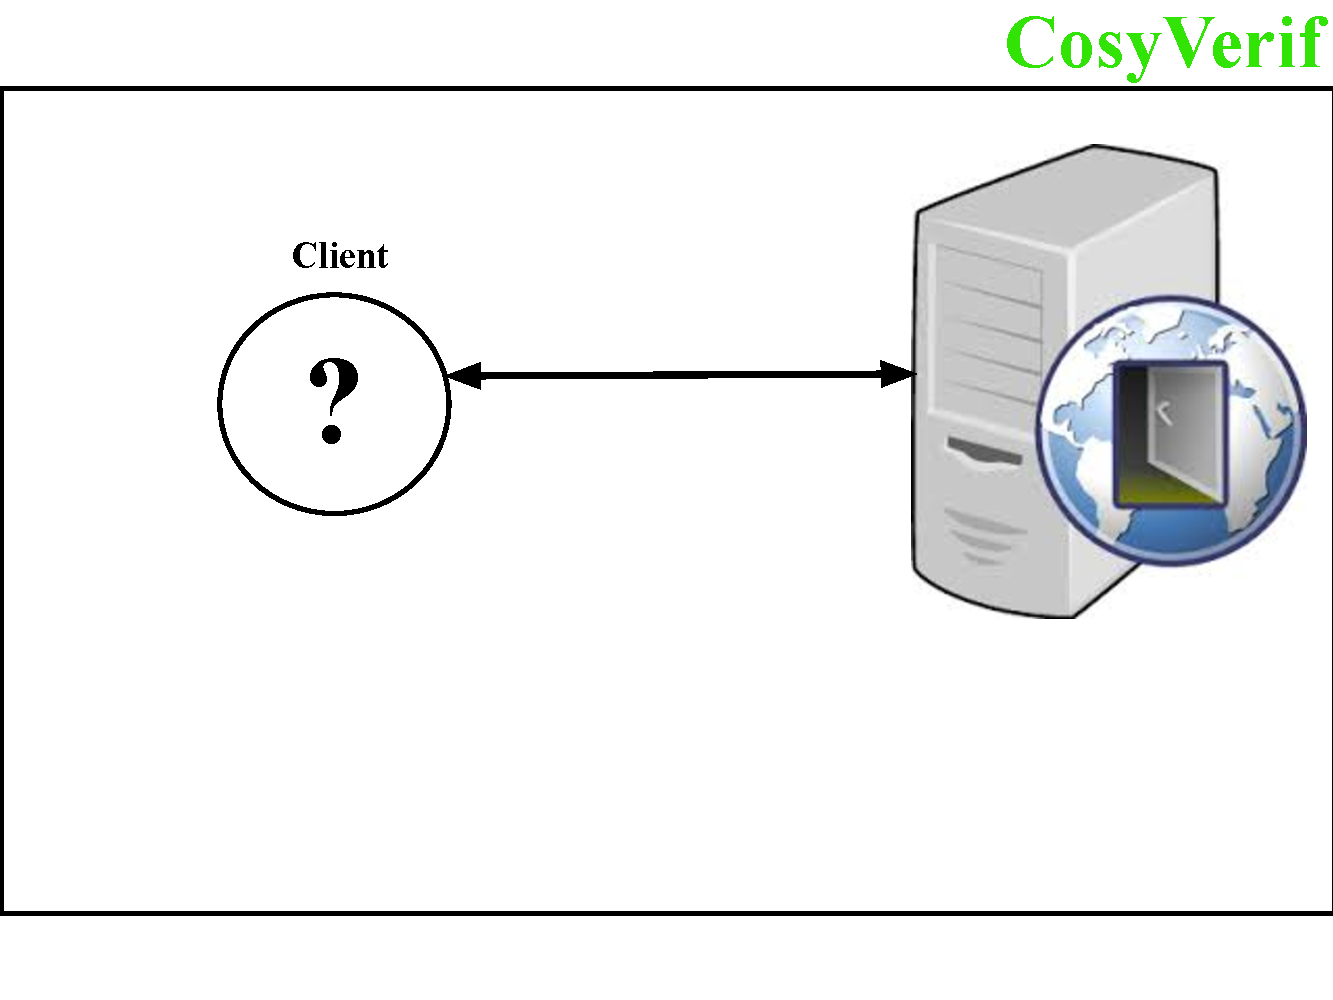
\includegraphics[width=10.5cm, height=4cm]{img/1-objectif}};
                 \end{tikzpicture}
            }%
            
            \only <2>{%
                \begin{tikzpicture}
                      \node
                          [anchor=north]
                          at (0,0)
                          {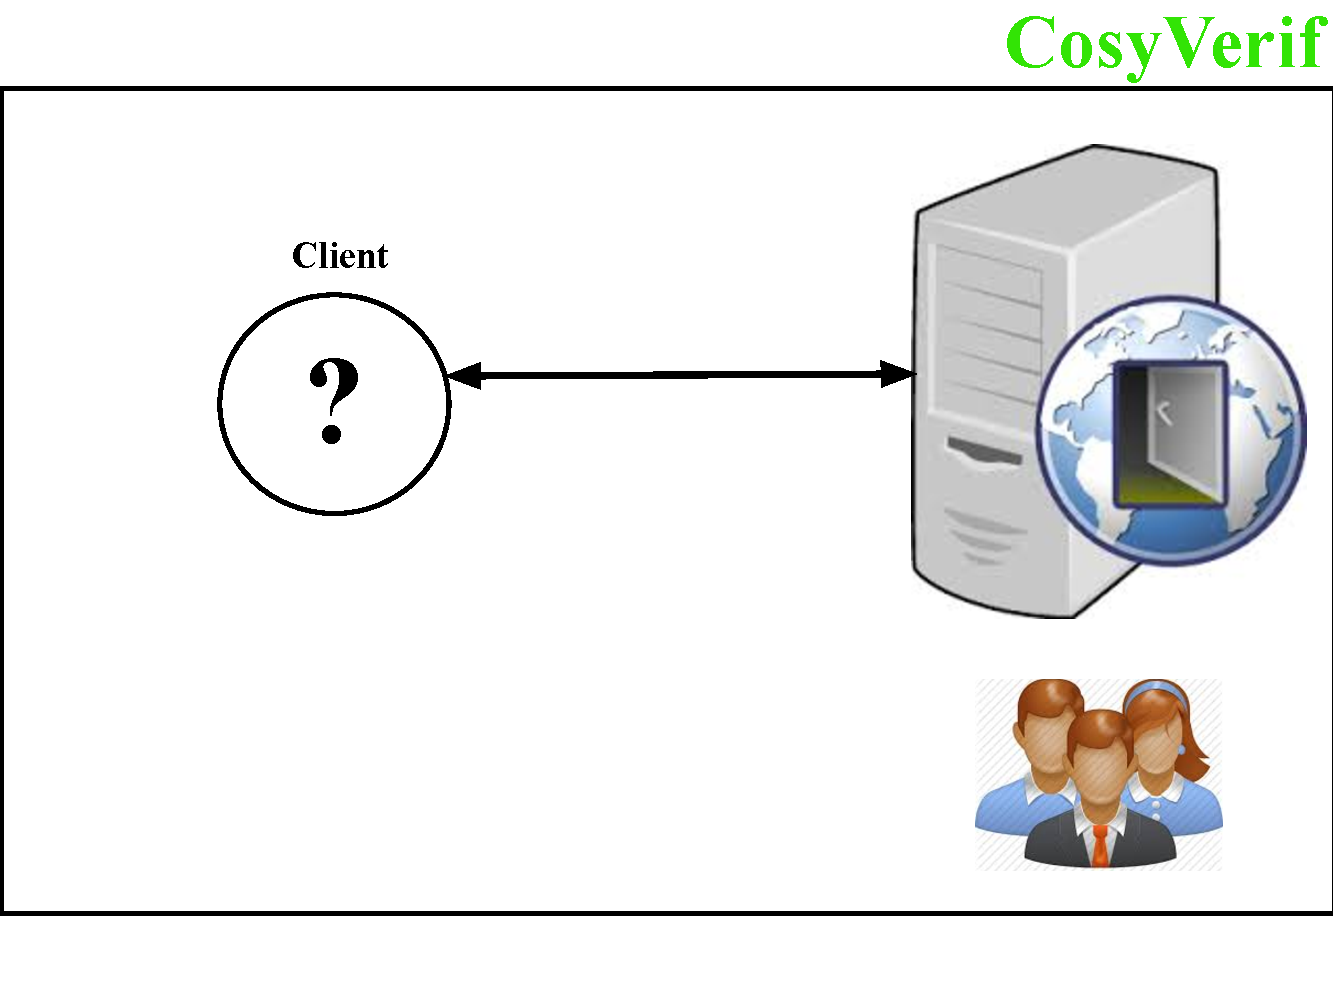
\includegraphics[width=10.5cm, height=4cm]{img/2-objectif}};
                 \end{tikzpicture}
            }%
            
            \only <3>{%
                \begin{tikzpicture}
                      \node
                          [anchor=north]
                          at (0,0)
                          {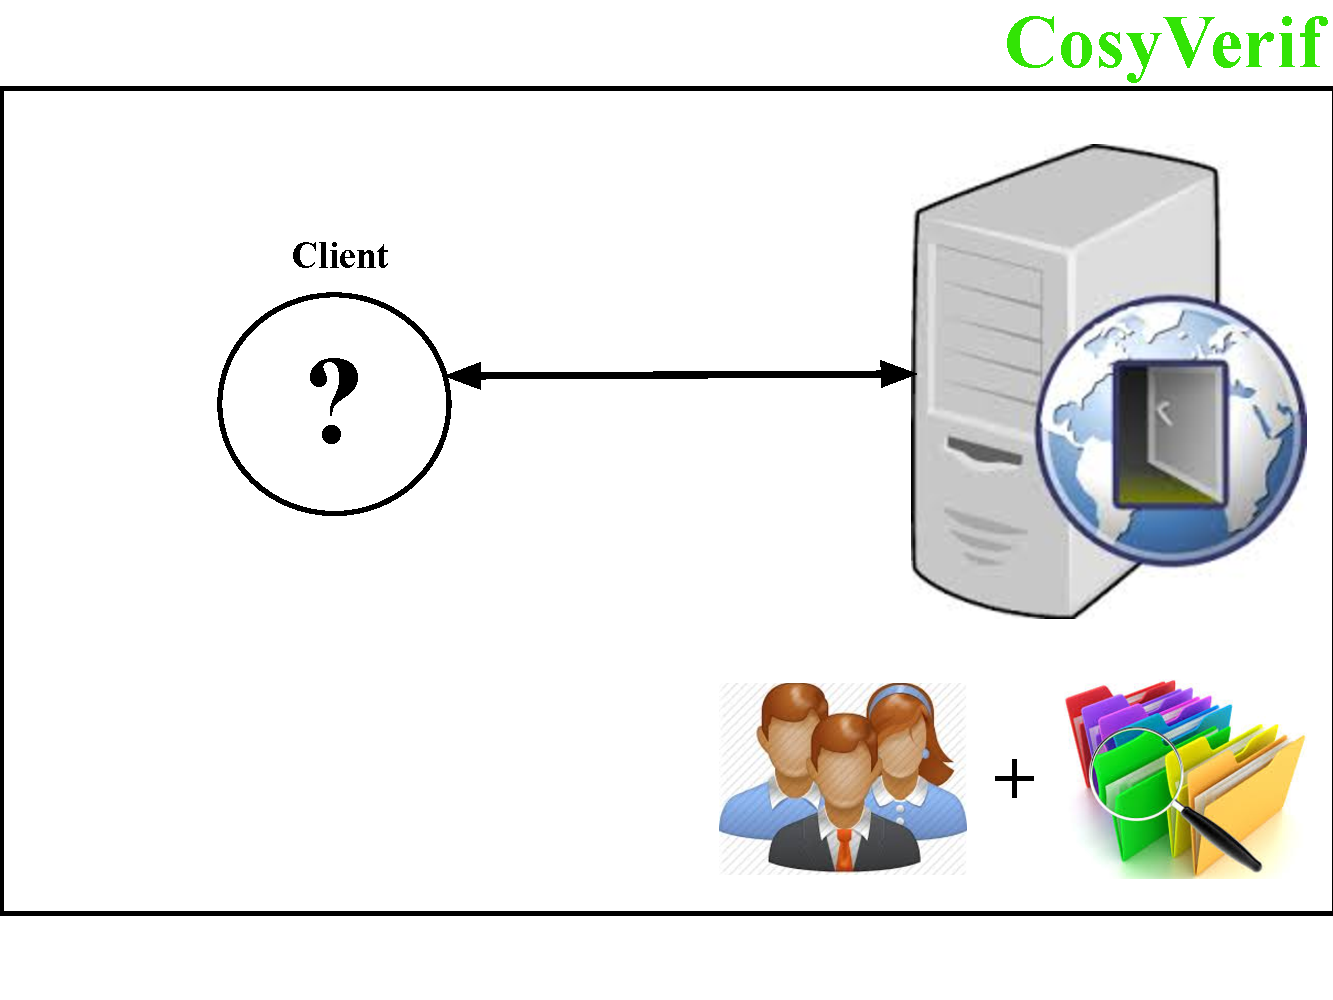
\includegraphics[width=10.5cm, height=4cm]{img/3-objectif}};
                 \end{tikzpicture}
            }%
            
            \only <4>{%
                \begin{tikzpicture}
                      \node
                          [anchor=north]
                          at (0,0)
                          {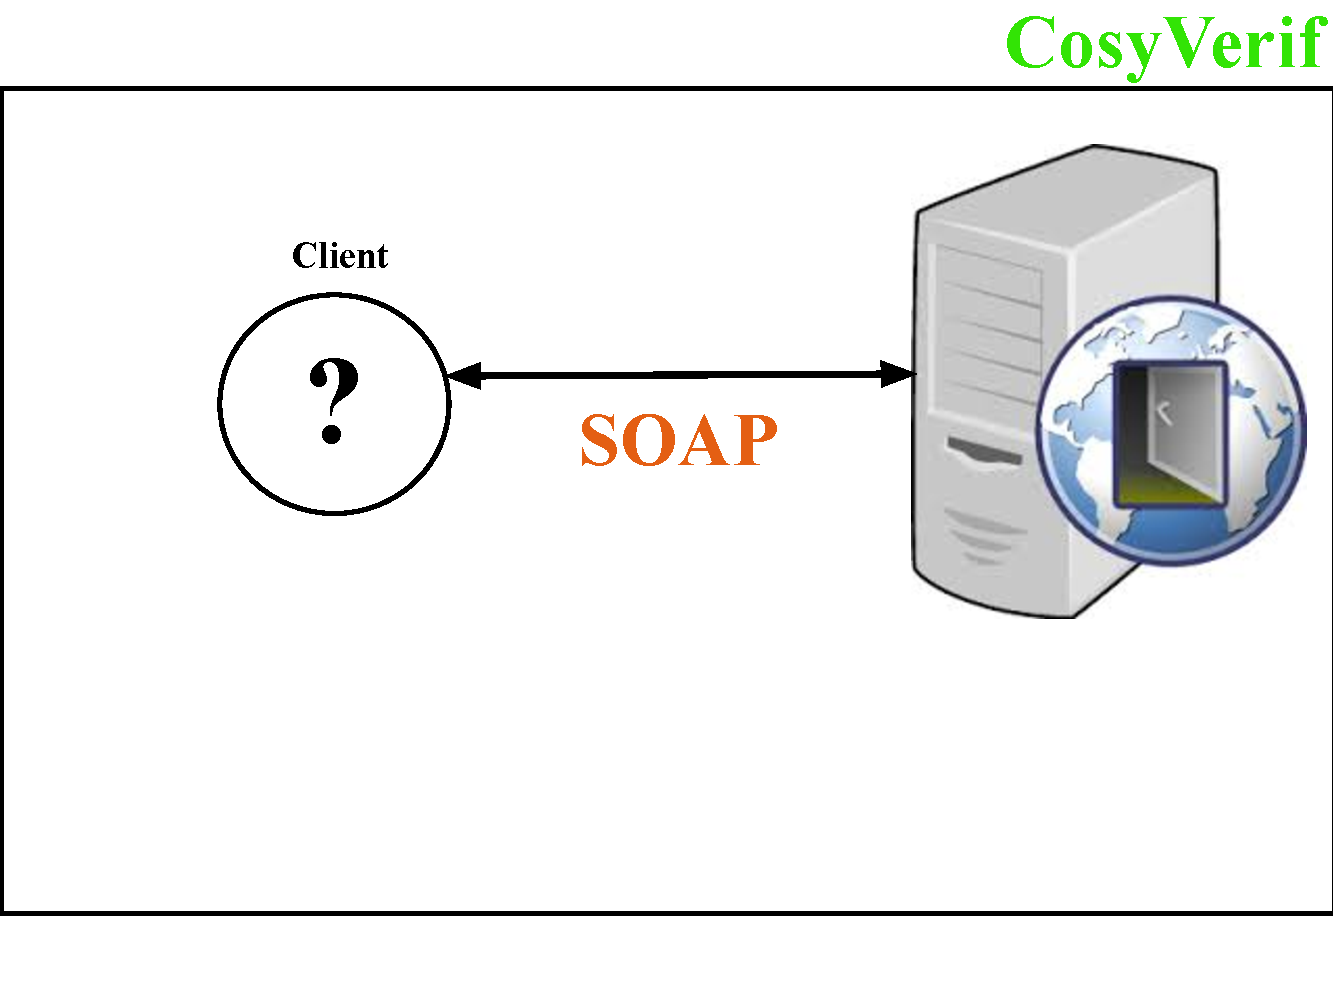
\includegraphics[width=10.5cm, height=4cm]{img/4-objectif}};
                 \end{tikzpicture}
            }%
            
            \only <5>{%
                \begin{tikzpicture}
                      \node
                          [anchor=north]
                          at (0,0)
                          {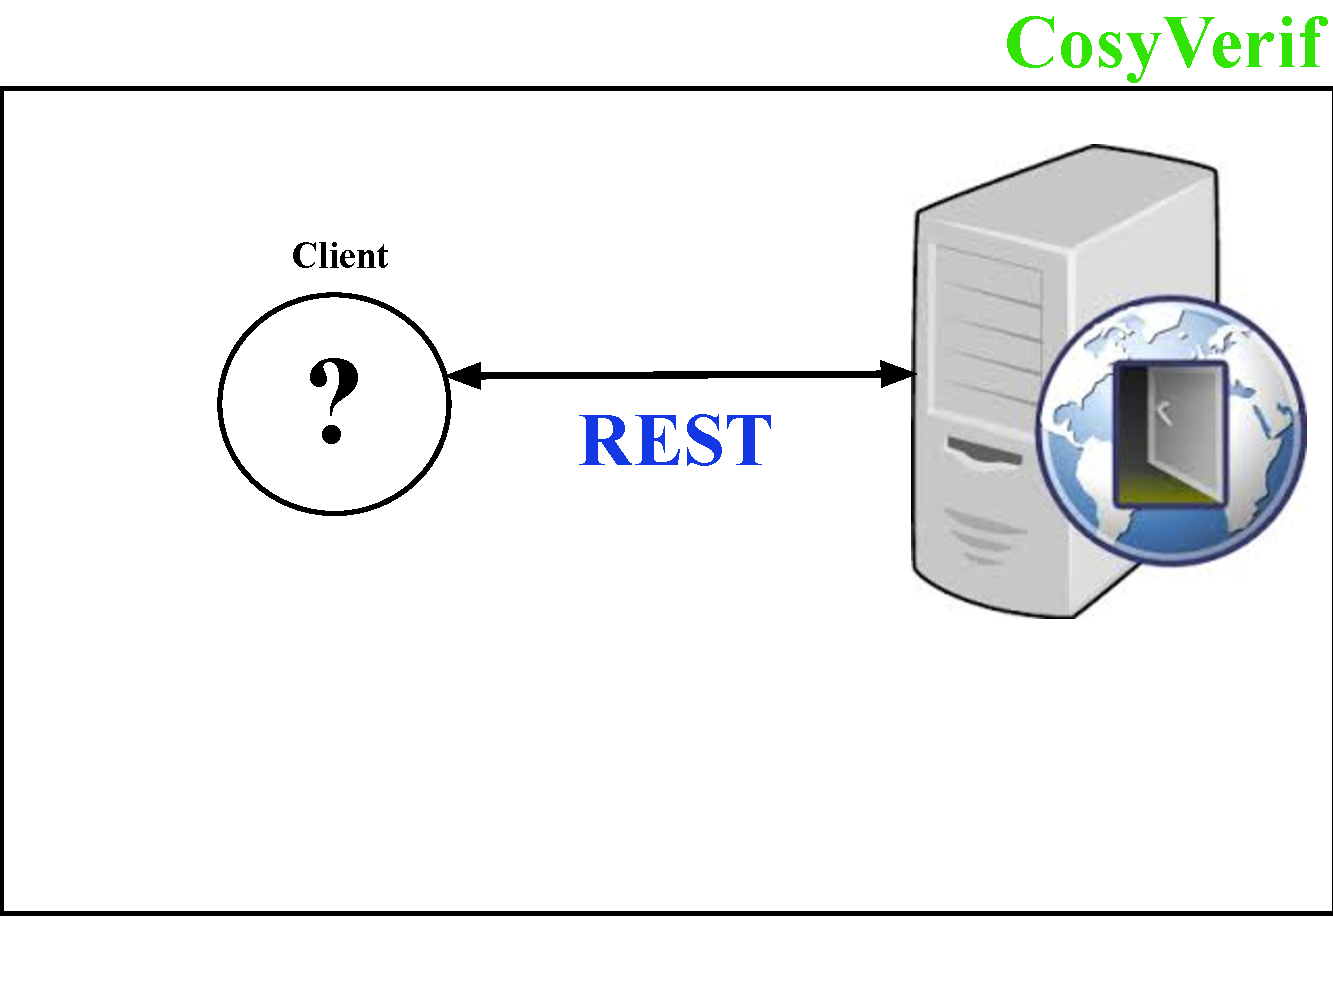
\includegraphics[width=10.5cm, height=4cm]{img/5-objectif}};
                 \end{tikzpicture}
            }%
            
            \only <6>{%
                \begin{tikzpicture}
                      \node
                          [anchor=north]
                          at (0,0)
                          {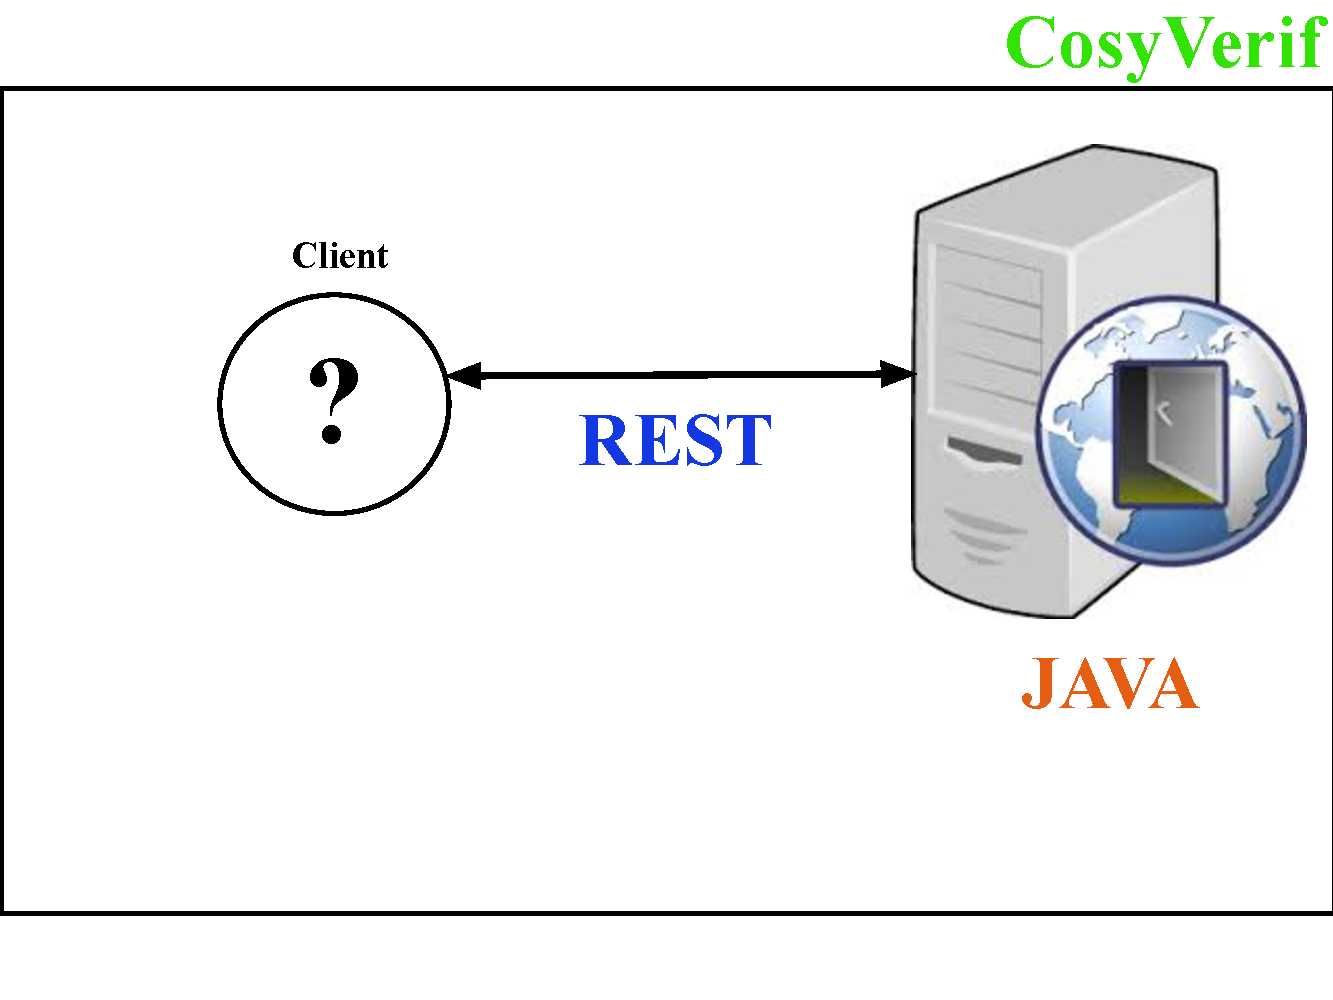
\includegraphics[width=10.5cm, height=4cm]{img/6-objectif}};
                 \end{tikzpicture}
            }%
            
            \only <7>{%
                \begin{tikzpicture}
                      \node
                          [anchor=north]
                          at (0,0)
                          {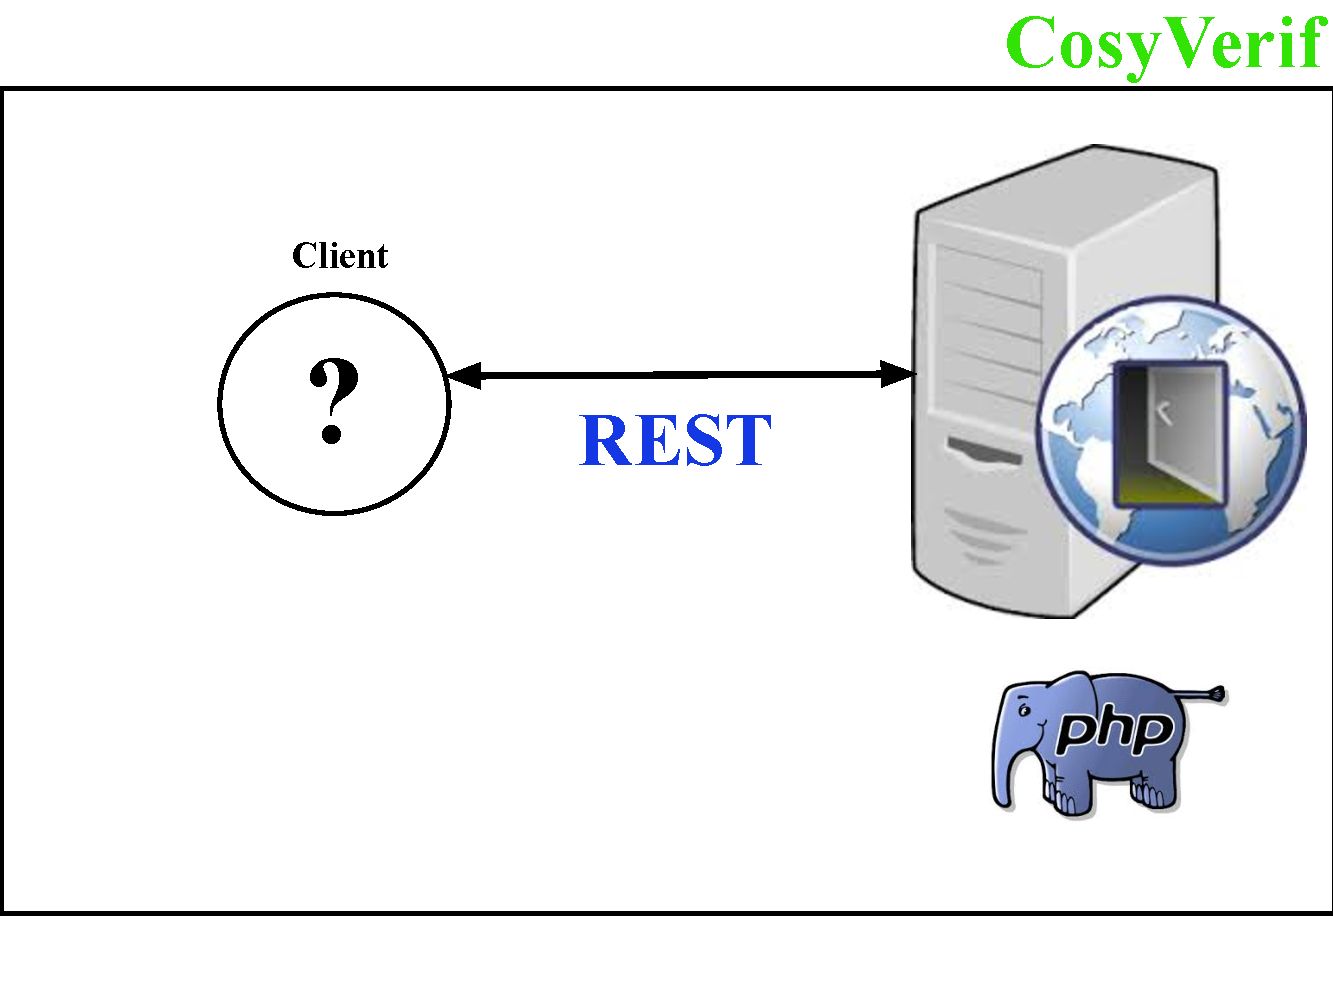
\includegraphics[width=10.5cm, height=4cm]{img/7-objectif}};
                 \end{tikzpicture}
            }%
            
            \only <8>{%
                \begin{tikzpicture}
                      \node
                          [anchor=north]
                          at (0,0)
                          {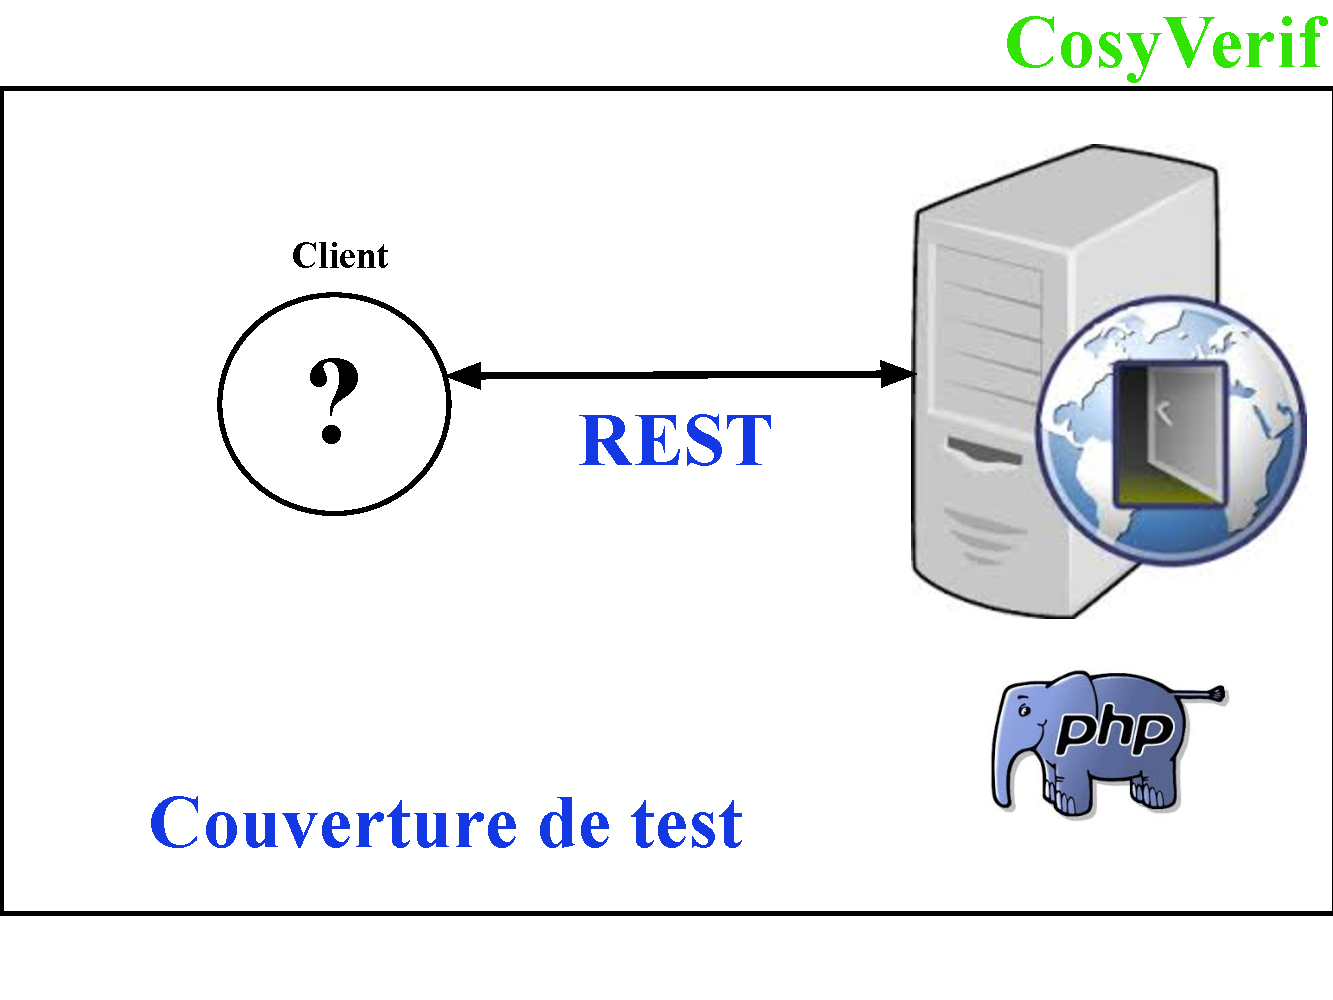
\includegraphics[width=10.5cm, height=4cm]{img/8-objectif}};
                 \end{tikzpicture}
            }%
 
    \end{minipage}
   
   \hrule
  
  \begin{minipage}{1\textwidth}
    
         \begin{itemize}
     	    \item <1-> Serveur maintenable
     	    \item <2-> Gestion des utilisateurs 
     	    \item <3-> Dépôt de modèles et de formalisms (comme PNMLWEB)
	    \item <4-> SOAP => REST (Representation State Transfert)
     	    \item <6-> JAVA => PHP 
     	    \item <8-> Test
         \end{itemize}
   \end{minipage}
 \end{frame}
 
    \begin{frame}[c]
  \frametitle{Arborescence utilisateurs}
  
  \begin{minipage}{1\textwidth}
  	\only <1-9>{%
                \begin{tikzpicture}
                      \node
                          [anchor=north]
                          at (0,0)
                          {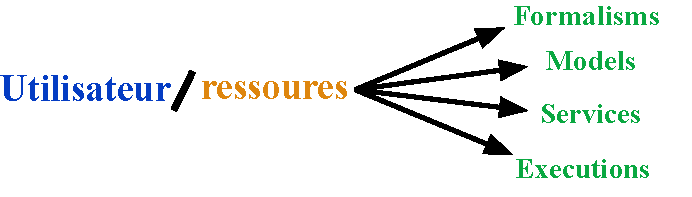
\includegraphics[width=10.5cm, height=4cm]{img/1-arbre-u}};
                 \end{tikzpicture}
            }%
            
            \only <10->{%
                \begin{tikzpicture}
                      \node
                          [anchor=north]
                          at (0,0)
                          {
\includegraphics[width=10.5cm, height=4cm]{img/2-arbre-u}};
                 \end{tikzpicture}
            }%
            
 
    \end{minipage}
   
   \hrule
  
  \begin{minipage}[t][15cm][t]{\textheight}
  
  \begin{columns}[T] % align columns
\begin{column}{.48\textwidth}
\only<2>{%
\lstinline!GET http://rest.cosyverif.org/users! \\
\lstinline!200 OK! \\
\lstinline!{ ... }!
}%
\only<3>{%
\lstinline!POST .../users/isokhona! \\
\lstinline!201 CREATED!
}%
\only<4>{%
\lstinline!POST .../users/alban! \\
\lstinline!201 CREATED!
}%

\only<5>{%
\lstinline!POST .../users/isokhona/models/model1! \\
\lstinline!201 CREATED!
}%

\only<6>{%
\lstinline!GET .../users/isokhona/models/model1! \\
\lstinline!200 OK & data!
}%

\only<7>{%
\lstinline!PUT .../users/isokhona/models/model1! \\
\lstinline!200 OK!
}%

\only<8>{%
\lstinline!DELETE .../users/isokhona/models/model1! \\
\lstinline!204 NO CONTENT!
}%

\only<9>{%
\lstinline!GET .../users/isokhona/models/model1! \\
\lstinline!410 GONE!
}%

\end{column}%
\hfill%
\begin{column}{.48\textwidth}
% http://www.texample.net/tikz/examples/filesystem-tree/
\tikzstyle{every node}=[draw=black,thick,anchor=west,minimum width=2cm,minimum height=2em]
\tikzstyle{selected}=[draw=red,fill=red!30]
\tikzstyle{optional}=[dashed,fill=gray!50]
\scriptsize
\begin{tikzpicture}[
every node={draw=black,thick,anchor=west},
selected={draw=red,fill=red!30},
grow via three points={one child at (-.5,-0.7) and
two children at (-.5,-0.7) and (-.5,-1.4)},
edge from parent path={(\tikzparentnode.south west) |- (\tikzchildnode.west)}]
\only<2->{
\node {/}
child { node {users} };
}
\end{tikzpicture}
\end{column}%
\end{columns}
    
   \end{minipage}
 \end{frame}
 
     \begin{frame}[c]
  \frametitle{Arborescence Projets}
  
  \begin{minipage}{1\textwidth}
  	\only <1>{%
                \begin{tikzpicture}
                      \node
                          [anchor=north]
                          at (0,0)
                          {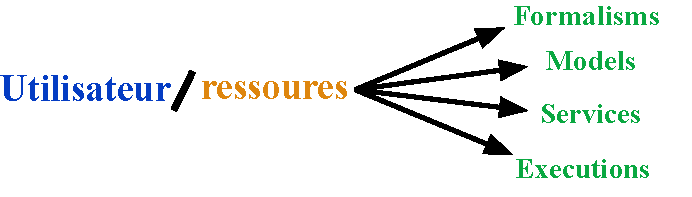
\includegraphics[width=10.5cm, height=4cm]{img/1-arbre-u}};
                 \end{tikzpicture}
            }%
            
            \only <2>{%
                \begin{tikzpicture}
                      \node
                          [anchor=north]
                          at (0,0)
                          {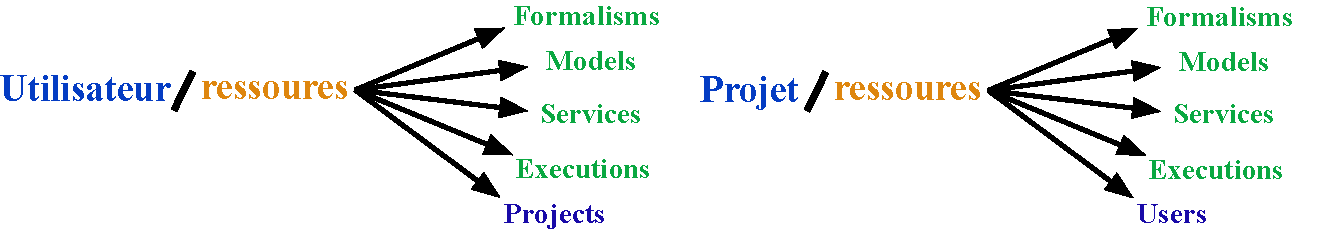
\includegraphics[width=10.5cm, height=4cm]{img/1-arbre-p}};
                 \end{tikzpicture}
            }%
            
            \only <3->{%
                \begin{tikzpicture}
                      \node
                          [anchor=north]
                          at (0,0)
                          {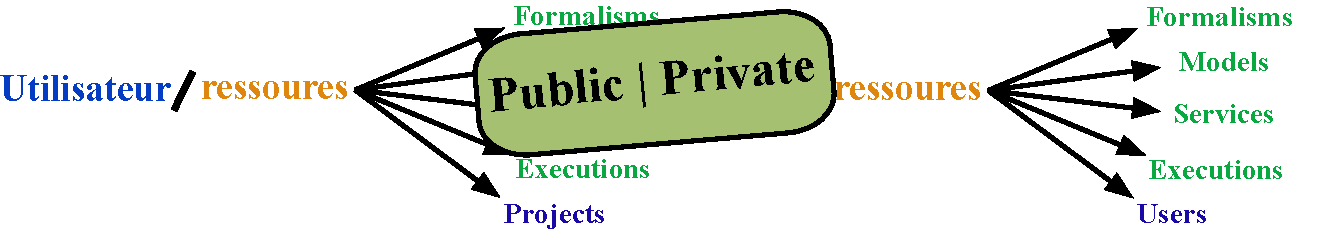
\includegraphics[width=10.5cm, height=4cm]{img/2-arbre-p}};
                 \end{tikzpicture}
            }%
            
 
    \end{minipage}
   
   \hrule
  
  \begin{minipage}[t][15cm][t]{\textheight}
  
  \begin{columns}[T] % align columns
\begin{column}{.48\textwidth}
\only<2->{%
\lstinline!GET http://rest.cosyverif.org/users! \\
\lstinline!200 OK! \\
\lstinline!{ ... }!
}%

\end{column}%
\hfill%
\begin{column}{.48\textwidth}
% http://www.texample.net/tikz/examples/filesystem-tree/
\tikzstyle{every node}=[draw=black,thick,anchor=west,minimum width=2cm,minimum height=2em]
\tikzstyle{selected}=[draw=red,fill=red!30]
\tikzstyle{optional}=[dashed,fill=gray!50]
\scriptsize
\begin{tikzpicture}[
every node={draw=black,thick,anchor=west},
selected={draw=red,fill=red!30},
grow via three points={one child at (-.5,-0.7) and
two children at (-.5,-0.7) and (-.5,-1.4)},
edge from parent path={(\tikzparentnode.south west) |- (\tikzchildnode.west)}]
\only<2->{
\node {/}
child { node {projects} }
child { node {users} };
}
\end{tikzpicture}
\end{column}%
\end{columns}
    
   \end{minipage}
 \end{frame}
 
 
\begin{frame}[c]
  \frametitle{Implémentation}
  
  \begin{minipage}{1\textwidth}
  	\only <1>{%
                \begin{tikzpicture}
                      \node
                          [anchor=north]
                          at (0,0)
                          {
\includegraphics[width=10.5cm, height=4cm]{img/1-implementation}};
                 \end{tikzpicture}
            }%
            
            \only <2->{%
                \begin{tikzpicture}
                      \node
                          [anchor=north]
                          at (0,0)
                          {
\includegraphics[width=10.5cm, height=4cm]{img/2-implementation}};
                 \end{tikzpicture}
            }%

             
    \end{minipage}
   
   \hrule
  
  \begin{minipage}{1\textwidth}
    
         \begin{itemize}
     	    \item <1-> Technologies
     	    \item <2-> Test
         \end{itemize}
   \end{minipage}
 \end{frame}
 
 
\begin{frame}[c]

\begin{center}

\par
\Huge Perspectives \& Conclusion

\end{center}
  
\end{frame}

\begin{frame}[c]
  \frametitle{Problématique/Objectif}
  
  \begin{minipage}{1\textwidth}
  	\only <1>{%
                \begin{tikzpicture}
                      \node
                          [anchor=north]
                          at (0,0)
                          {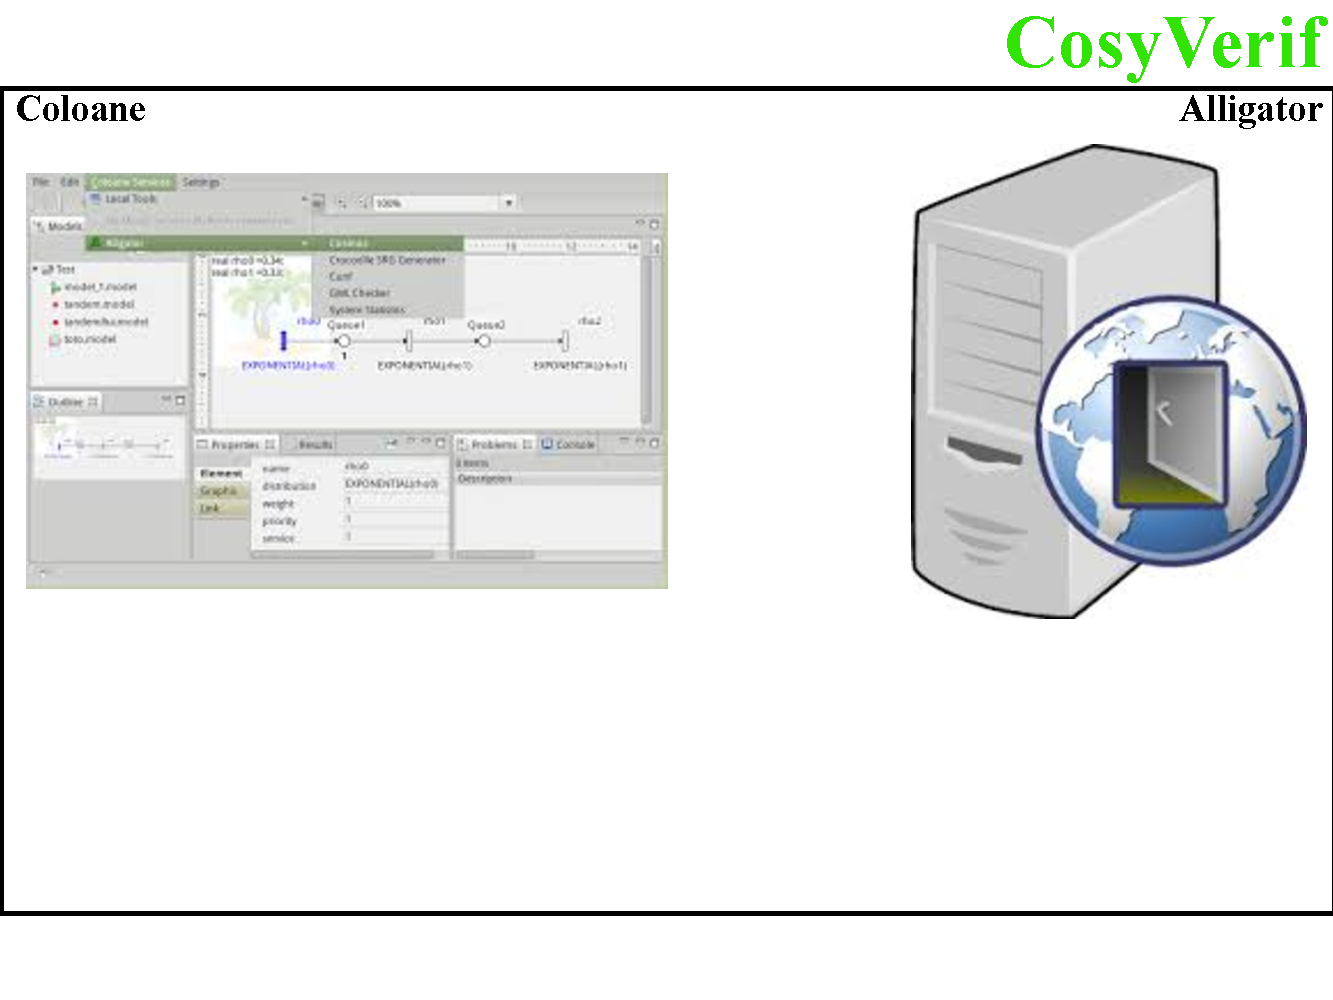
\includegraphics[width=10.5cm, height=4cm]{img/1-probleme}};
                 \end{tikzpicture}
            }%
            
            \only <2->{%
                \begin{tikzpicture}
                      \node
                          [anchor=north]
                          at (0,0)
                          {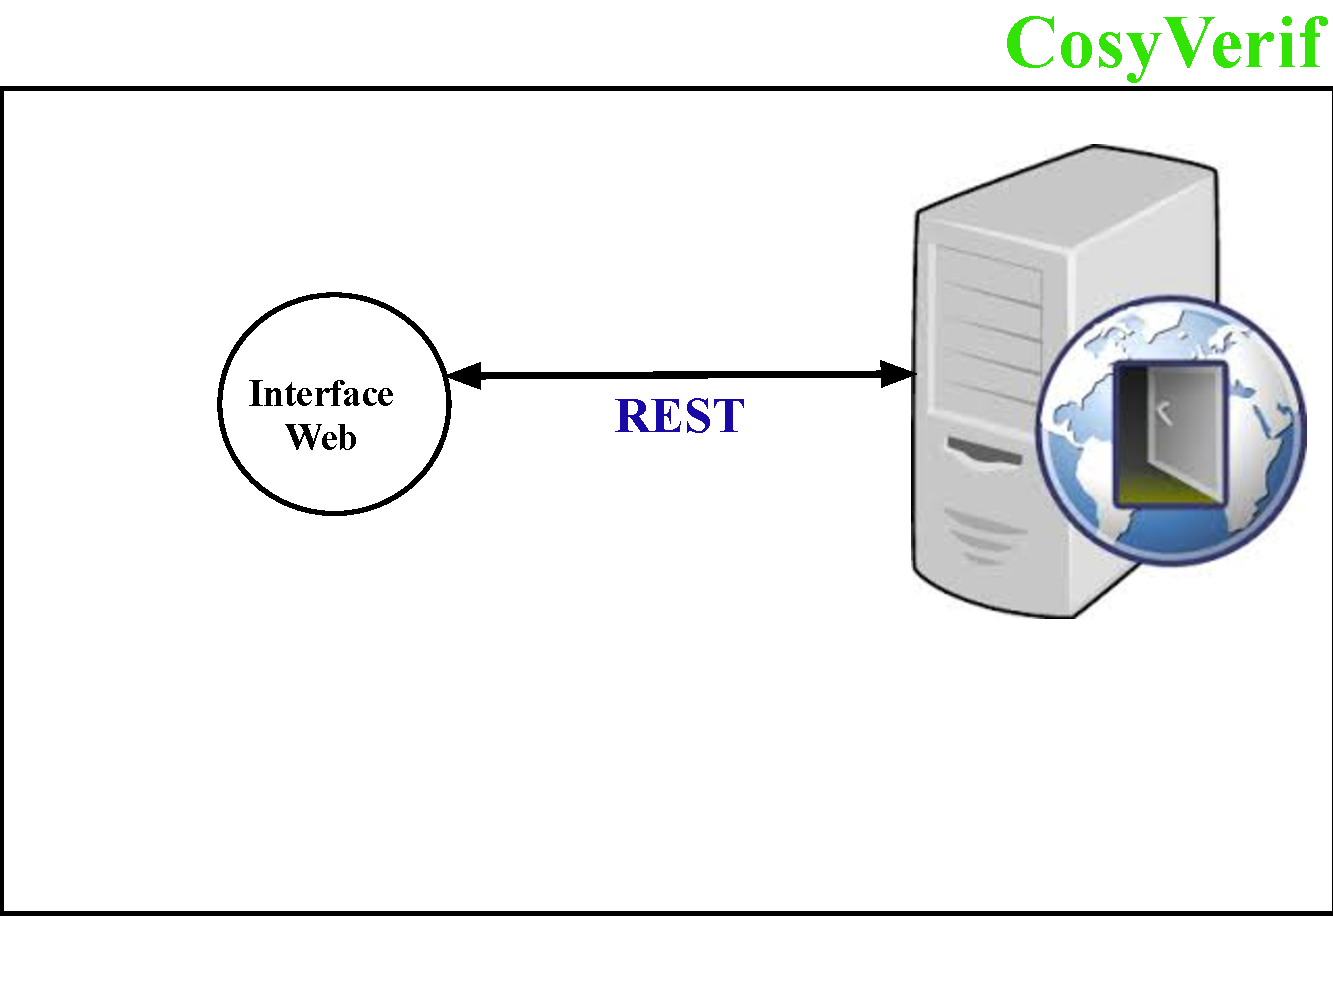
\includegraphics[width=10.5cm, height=4cm]{img/1-client}};
                 \end{tikzpicture}
            }%

             
    \end{minipage}
   
   \hrule
  
  \begin{minipage}{1\textwidth}
    
         \begin{itemize}
     	    \item <1-> Maintenance
     	    \item <1-> Fonctionnalités
	    \item <1-> Evolution
	    \item <2-> Nouvelle interface web
         \end{itemize}
   \end{minipage}
 \end{frame}
 
 
\begin{frame}[c]
  \frametitle{Interface web}
 
 \begin{columns}[T] % align columns
\begin{column}{.25\textwidth}
\only<1-2>{%
\textsf{Create user}
}%

\only<3>{%
\textsf{Create resource}
}%


\only<4>{%
\textsf{Create project}
}%

\only<5>{%
\textsf{Create invitation}
}%

\only<6>{%
\textsf{Search}
}%

\end{column}%
\hfill%
\begin{column}{.81\textwidth}

	\only <1>{%
                \begin{tikzpicture}
                      \node
                          [anchor=north]
                          at (0,0)
                          {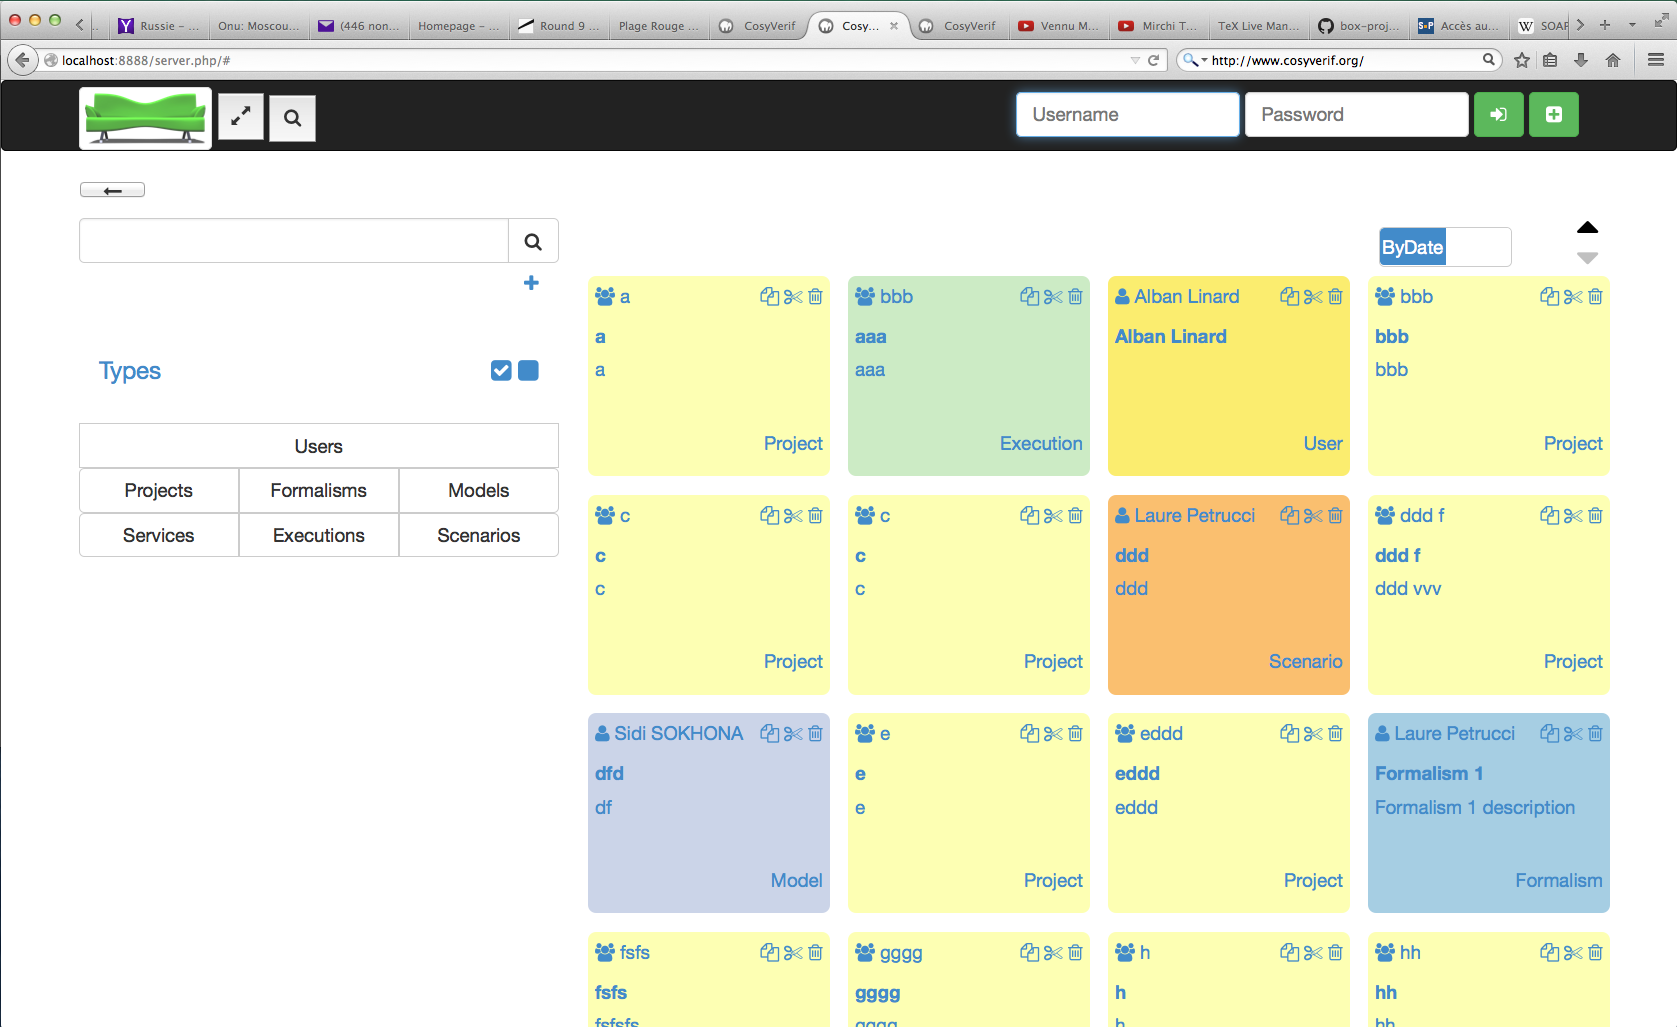
\includegraphics[width=8cm, height=10cm]{img/1-ecran-create-user}};
                 \end{tikzpicture}
            }%
            
            \only <2>{%
                \begin{tikzpicture}
                      \node
                          [anchor=north]
                          at (0,0)
                          {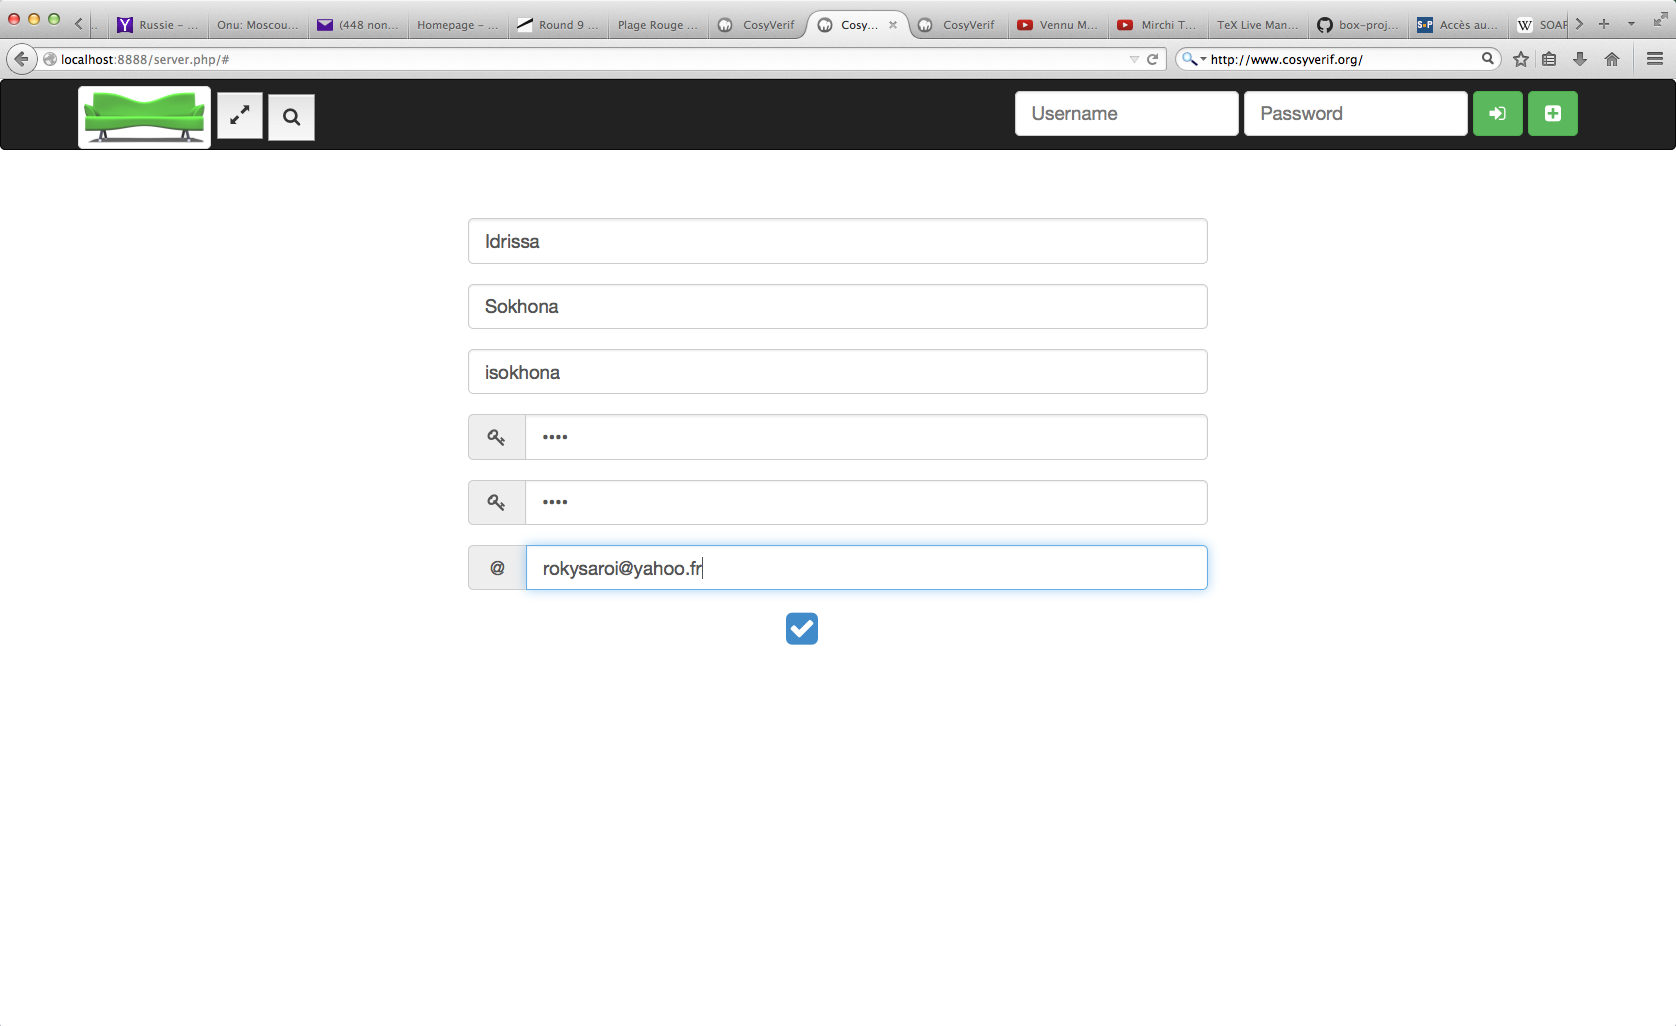
\includegraphics[width=8cm, height=10cm]{img/2-ecran-create-user}};
                 \end{tikzpicture}
            }%
\end{column}%
\end{columns}
 
  
\end{frame}

\begin{frame}[c]
  \frametitle{Implémentation}
  
  \begin{minipage}{1\textwidth}
  	\only <1->{%
                \begin{tikzpicture}
                      \node
                          [anchor=north]
                          at (0,0)
                          {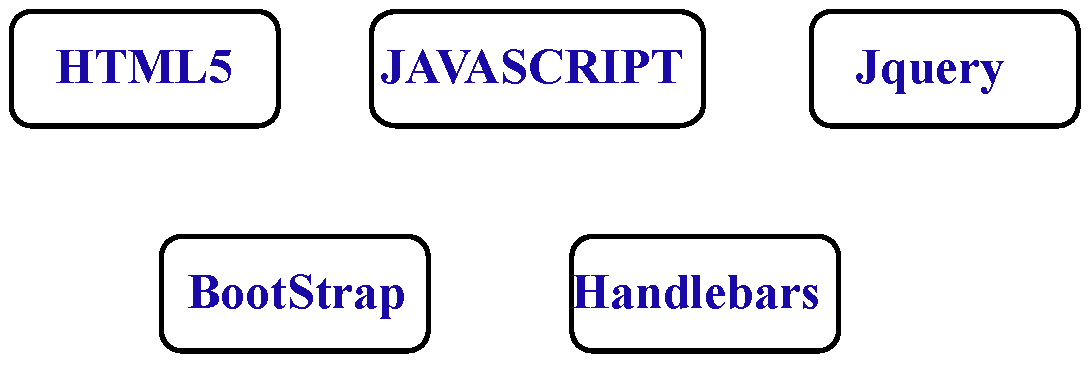
\includegraphics[width=10.5cm, height=4cm]{img/1-implementation-client}};
                 \end{tikzpicture}
            }%
            
    \end{minipage}
   
   \hrule
  
  \begin{minipage}{1\textwidth}
    
         \begin{itemize}
     	    \item <1-> Technologies
         \end{itemize}
   \end{minipage}
 \end{frame}
 
\begin{frame}[c]
\par
\Huge Perspectives \& Conclusion
\end{frame}

\begin{frame}[c]
  \frametitle{Bilan}
  
  \begin{minipage}{1\textwidth}
  	
\begin {center}
	\par
	\Huge Bilan
\end{center}
             
    \end{minipage}
   
   \hrule
  
  \begin{minipage}{1\textwidth}
    
         \begin{itemize}
     	    \item <1-> Serveur
     	    \item <2-> Interface web
	    \item <3-> Personnel
         \end{itemize}
   \end{minipage}
\end{frame}

\begin{frame}[c]

\begin{center}

\par
\Huge Question ?

\end{center}
\end{frame}

\end{document}
